This study is focused on predicting which antibiotics will be resisted by a strain of \textit{Escherichia coli} from the strain's genomic data. For this, we used a well-defined pipeline. We first assembled a large public data set that provided the genomic variation in thousands of \textit{E. coli} strains, along with the laboratory resistance phenotypes~\cite{arcadia2024}. Next, we prepared the data to be used for modelling. First, records from the three source files were matched. The laboratory data was then converted to numbers. If a strain and drug combination had not been previously evaluated, then a mask was applied. A guessed value was not placed in it. From the cleaned data we generated three complementary genomic views: single-nucleotide polymorphism (SNP) blocks grouped by gene, a gene presence and absence profile and per-gene summary statistics. We then implemented a hybrid architecture, TriLens-MoE-Stack, where three specialised neural lenses compute these views, a mixture-of-experts gate combines them and their result is added to five classical base learners via a logistic-regression meta-learner. Lastly, we considered each component using precision-recall AUC and clinical error rates. Three data splits were tested: random, phylogroup-stratified and sequence-type lineage hold-out. The method was also validated using an independent data set. In summary, the pipeline proceeds one step at a time, starting with the collection and purification of genomic data, then creating a model that can predict resistance to seven antibiotics simultaneously and is interpretable and fairly assessed.

\section{Top-Level Overview of the Proposed System}

\begin{figure}[H]
  \centering
  \begin{adjustbox}{max width=\textwidth, max height=0.92\textheight, center}
  
% =====================================================================
%  Figure 4.1 -- Overview of the proposed system  (REVISED)
%  This is your own TikZ picture with the agreed corrections applied.
%  Nothing outside the picture changed: same macros (\PNBlock, \PNCaption,
%  \DNA, \Broom, ...), same styles (dashedPanel, panelTitle, card, arrow,
%  orangeArrow, redArrow, greenArrow), same colours.
%
%  WHAT CHANGED (search for "CHANGED:" to find each edit in place)
%   1. Pre-processing panel: "Cleaning + deduplication", "Normalization
%      Z=(X-mu)/sigma" and "Feature reduction: constant + correlation
%      filter" all removed -- none of the three is in the thesis.
%      Replaced by record matching, phenotype encoding and the label mask.
%   2. NEW Gene Selection band placed AFTER the split, fed by all three
%      protocols -- this is the leakage-order fix.
%   3. Data Split panel + strategy cards carry the real per-split sizes,
%      including the lineage holdout's 4,836 / 1,081 / 1,045.
%   4. Lens B is labelled strain-conditioned.
%   5. All four evaluation pillars are present and numbered; a new
%      Interpretability panel is added.
%   6. GeneAttentionNet becomes a design-lineage note; PR-AUC 0.769 gone,
%      and the misleading arrow from Lens C is removed.
%   7. Giessen: 90.4% -> 90.0%, and "same TriLens methodology" corrected
%      to the classical stacking arm only.
%   8. The three coloured split arrows now converge on one place instead
%      of running unlabelled to every block, and a legend is given.
%
%  Block contents were kept to short labels -- the detail belongs in the
%  Chapter 4 prose, not in the workflow figure. Bounding box: -44.50 ->
%  -45.20, aspect ratio 1.57 -> 1.60, so the float still fits its page.
% =====================================================================
 
\begin{tikzpicture}[x=1cm,y=1cm,scale=.82,transform shape]
\renewcommand{\Huge}{\fontsize{28.5}{34}\selectfont}
\tikzset{
  arrow/.append style={shorten >=1.2pt, rounded corners=2pt},
  orangeArrow/.append style={shorten >=1.2pt, rounded corners=2pt},
  redArrow/.append style={shorten >=1.2pt, rounded corners=2pt},
  greenArrow/.append style={shorten >=1.2pt, shorten <=0.5pt, rounded corners=2pt},
  % Small numbered "stage" badges + zone corner tags used to make the
  % top-to-bottom reading order of the redesigned pipeline explicit.
  stageBadge/.style args={#1}{circle,fill=#1,text=white,draw=black!25,
    line width=.5pt,font=\bfseries\Large,minimum size=1.05cm,inner sep=0pt},
  zoneTag/.style args={#1}{font=\bfseries\Huge,text=#1!65!black,anchor=west},
}
 
% CHANGED: bounding box nudged to fit the new gene-selection band.
\path[use as bounding box] (-1.00,-45.20) rectangle (45.70,30.30);
 
% Shift the complete pipeline upward while retaining all internal alignments.
\begin{scope}[yshift=1.5cm]
 
% =====================================================================
% Dataset panel
% =====================================================================
\begin{scope}[xshift=2.30cm,yshift=.5cm]
\node[
  dashedPanel,
  draw=navy,
  minimum width=11.6cm,
  minimum height=11.10cm
] (datasetBox) at (3.20,22.25) {};
 
\node[panelTitle,text=navy,anchor=north,font=\bfseries\Huge]
  at (3.20,27.25) {Dataset};
 
\node[font=\bfseries\Huge,align=center]
  at (3.20,25.05) {Arcadia E. coli\\AMR dataset};
 
\DNA{(0.30,19.35)}{1.8}
 
\foreach \x/\y/\c in {
  2.05/23.48/blueedge,
  2.72/23.68/orangeedge,
  3.35/23.10/navy,
  4.05/23.48/orangeedge,
  4.70/23.20/blueedge,
  5.18/23.58/orangeedge,
  1.82/22.55/orangeedge,
  2.62/22.28/blueedge,
  3.40/22.52/blueedge,
  4.12/22.60/orangeedge,
  4.78/22.35/navy,
  5.28/22.82/blueedge,
  2.12/21.72/navy,
  3.18/21.82/orangeedge,
  4.18/21.76/blueedge%
}{
  \fill[fill=\c] (\x,{\y-1.5}) circle (.10);
}
 
\Bacteria{(5.00,20.15)}{2}
 
% CHANGED: the two source deposits are flagged, because they feed two
% different views. Only "Release 2" is a name the thesis uses (Section
% 4.3.2.2); the variant-call deposit is left unnamed rather than guessed at.
\node[font=\Huge,align=center] at (3.20,17.75) {6,962 genomes};
\end{scope}
 
% =====================================================================
% Pre-processing panel
% CHANGED: this panel used to read "Cleaning + deduplication / duplicates
% removed", "Normalization Z=(X-mu)/sigma" and "Feature reduction:
% constant + correlation filter". None of those three appears anywhere in
% the thesis: Section 4.3.1 says the genomes needed no cleaning, no
% z-scoring is described, and the real filters are the two in Section
% 4.3.4 (which have now moved below the split, where they belong).
% =====================================================================
\begin{scope}[xshift=7.55cm,yshift=.5cm]
\node[
  rounded corners=2mm,
  draw=orangeedge!60,
  fill=orangefill!28,
  line width=.7pt,
  minimum width=14.5cm,
  minimum height=11.10cm
] (preBox) at (13,22.25) {};
 
\node[panelTitle,text=navy,anchor=north,font=\bfseries\Huge,align=center]
  at (13,27.25) {Preprocessing\\Framework};
 
\node[
  card=orangeedge,
  minimum width=13.5cm,
  minimum height=2.0cm
] (matchCard) at (13,23.35) {
  \bfseries\Huge{Record matching}\\[4pt]
  \Huge three files intersected
};
 
\node[
  card=orangeedge,
  minimum width=13.5cm,
  minimum height=2.0cm
] (labelCard) at (13,20.65) {
  \bfseries\Huge{Phenotype encoding}\\[4pt]
  \Huge R, I $\rightarrow$ 1 \quad S $\rightarrow$ 0
};
 
\node[
  card=orangeedge,
  minimum width=13.5cm,
  minimum height=2.0cm
] (maskCard) at (13,18.15) {
  \bfseries\Huge{Label mask}\\[4pt]
  \Huge $6{,}962\times7$
};
 
\Broom{(6.55,22.55)}{.85}
\Bars{(6.55,20.15)}{.85}
\Funnel{(6.55,17.95)}{.75}
\end{scope}
 
\draw[arrow] (datasetBox.east) -- (preBox.west);
 
% =====================================================================
% Data split panel
% =====================================================================
\begin{scope}[xshift=12.25cm,yshift=.5cm]
\node[
  rounded corners=2mm,
  draw=blueedge!60,
  fill=bluefill!48,
  line width=.7pt,
  minimum width=14.5cm,
  minimum height=11.10cm
] (splitPanelBox) at (24.8,22.25) {};

\node[panelTitle,text=navy,anchor=north,font=\bfseries\Huge,align=center]
  at (24.8,27.25) {Data Split\\Framework};

\node[
  card=blueedge,
  minimum width=12.6cm,
  minimum height=2.0cm
] (training) at (24.8,23.25) {
  \bfseries\Huge{Training (70\%)}\\[2pt]
  \Huge 4,872 genomes
};

\node[
  card=blueedge,
  minimum width=12.6cm,
  minimum height=2.0cm
] (validation) at (24.8,20.7) {
  \bfseries\Huge{Validation (15\%)}\\[2pt]
  \Huge 1,045 genomes
};

\node[
  card=blueedge,
  minimum width=12.6cm,
  minimum height=2.0cm
] (testing) at (24.8,18.2) {
  \bfseries\Huge{Testing (15\%)}\\[2pt]
  \Huge 1,045 genomes
};

\GradCap{(19,22.85)}{.85}
\Clipboard{(19,20.3)}{.85}
\Clipboard{(19,17.8)}{.75}


\end{scope}

\node[
  minimum width=12.9cm,
  minimum height=8.9cm,
  inner sep=0pt
] (splitBox) at (31.1,22.1) {};

% Data-splitting strategies
\node[
  card=blueedge,
  minimum width=6.6cm,
  minimum height=2.15cm,
  font=\bfseries\Huge
] (randomSplit) at ([xshift=-8.2cm,yshift=-3cm]splitBox.south) {
  Random Split
};

\node[
  card=blueedge,
  minimum width=7.6cm,
  minimum height=2.15cm,
  font=\bfseries\Huge
] (phylogroupSplit) at ([yshift=-3cm]splitBox.south) {
  Phylogroup-\\Stratified
};

\node[
  card=blueedge,
  minimum width=7.2cm,
  minimum height=2.15cm,
  font=\bfseries\Huge
] (lineageHoldout) at ([xshift=8.2cm,yshift=-3cm]splitBox.south) {
  Lineage\\Holdout
};

% One shared trunk from the centre of the Data Split panel's bottom edge,
% forked to the three splitting strategies. Pin the start to the panel frame
% explicitly so it cannot appear to originate from the Testing card.
\coordinate (splitStrategyStart) at
  (splitPanelBox.south);
\coordinate (splitStrategyFork) at
  ([yshift=-0.5cm]splitStrategyStart);
\draw[line] (splitStrategyStart) -- (splitStrategyFork);
\draw[line]
  (randomSplit.north |- splitStrategyFork) --
  (lineageHoldout.north |- splitStrategyFork);
\draw[arrow]
  (randomSplit.north |- splitStrategyFork) -- (randomSplit.north);
\draw[arrow]
  (phylogroupSplit.north |- splitStrategyFork) -- (phylogroupSplit.north);
\draw[arrow]
  (lineageHoldout.north |- splitStrategyFork) -- (lineageHoldout.north);

\draw[arrow] (preBox.east) -- (splitPanelBox.west |- preBox.east);
 
% =====================================================================
% CHANGED -- NEW STAGE: gene selection, AFTER the split.
%
% This is the single most important correction. The old figure put
% "Feature reduction" inside the pre-processing panel, i.e. BEFORE the
% split, which is exactly the leaked pipeline the thesis says it found and
% fixed (Section 4.3.5: "re-fitted on each split's training partition
% instead of being computed only once ... The definition of the pipeline
% used an earlier version that leaked information between splits, which
% was fixed prior to any results in this thesis").
% =====================================================================
\PNBlock{stage15}{(25.8,10.5)}{30cm}{2.70cm}{orangefill}{orangeedge}{
  \Huge\textbf{Gene Selection}\\[5pt]
  \Huge $\ge$ 5 SNPs $\rightarrow$ 13,799 genes
  \quad$\bullet$\quad
  XGBoost gain $\rightarrow$ \textbf{top 5,000 genes}
}
 
 
% Straight arrows carry the three split protocols into gene selection.
\draw[arrow]
  (randomSplit.south) -- (randomSplit.south |- stage15.north);
\draw[greenArrow]
  (phylogroupSplit.south) -- (phylogroupSplit.south |- stage15.north);
\draw[redArrow]
  (lineageHoldout.south) -- (lineageHoldout.south |- stage15.north);
 
% =====================================================================
% Genomic input blocks
% CHANGED: pushed down to make room for the gene-selection band, and now
% fed from it rather than straight from the split.
% =====================================================================
\def\genomicViewWidth{5cm}
\def\genomicViewHeight{4.15cm}
\coordinate (genomicViewRow) at ([yshift=-12.90cm]splitBox.south);
 
\PNBlock{snp}{([xshift=-8.2cm]genomicViewRow)}{\genomicViewWidth}{\genomicViewHeight}{bluefill}{blueedge}{
  \Huge\textbf{SNP}\\[3pt]
  \Huge\textbf{blocks}
}
\PNCaption{snp}{\Huge 6,962$\times$5,000$\times$64}
\DNA{([xshift=-2cm,yshift=-.62cm]snp.center)}{.60}
 
\PNBlock{gene}{(genomicViewRow)}{\genomicViewWidth}{\genomicViewHeight}{bluefill}{blueedge}{
  \Huge\textbf{Gene}\\[3pt]
  \Huge\textbf{Presence/}\\[3pt]
  \Huge\textbf{Absence}\\[3pt]
  \Huge\textbf{Matrix}
}
\PNCaption{gene}{\Huge 6,962$\times$32,441}
 
\PNBlock{summary}{([xshift=8.2cm]genomicViewRow)}{\genomicViewWidth}{\genomicViewHeight}{bluefill}{blueedge}{
  \Huge\textbf{Genomic}\\[4pt]
  \Huge\textbf{Summary}\\[4pt]
  \Huge\textbf{Stats}
}
\PNCaption{summary}{{\Huge 6,962$\times$5,000$\times$4}}
 
% Classical branch. CHANGED: its two distinct inputs are now named -- four
% learners read the gene-level features, XGB_raw reads the chi-squared
% prefiltered raw SNP matrix (Section 4.2.2, Table 4.8).
\PNBlock{ensemble}{([xshift=-8.5cm,yshift=-2.4cm]snp.west)}{11.3cm}{4.80cm}{orangefill}{orangeedge}{
  {\Huge\itshape Classical Arm}\\[3pt]
  \Huge\textbf{Classical ML Ensemble}\\[3pt]
  \Huge\textbf{5 base learners (OOF)}\\[4pt]
  \Huge XGB\_gene, LGBM, RF,\\[3pt]
  \Huge LogReg, XGB\_raw\\[3pt]
  \Huge XGB\_raw: $\chi^2$\\[3pt]
  \Huge top-50,000 raw SNPs
}
 
\node[font=\Huge,anchor=north]
  at ([yshift=-.28cm]ensemble.south) {(5-fold OOF)};
 
% CHANGED: gene selection feeds only the two views that are built from the
% selected 5,000 genes, plus the classical arm's gene-level feature matrix
% (Section 4.1, "the identical gene features feed five base learners";
% Figure 4.4 shows that matrix as 5,000 genes x 4 stats).
\draw[orangeArrow] (snp.north     |- stage15.south) -- (snp.north);
\draw[orangeArrow] (summary.north |- stage15.south) -- (summary.north);
\draw[orangeArrow] (11.9,0 |- stage15.south) -- ++(0,-0.7) -| (ensemble.north);
\node[font=\Huge,anchor=south,text=black!82]
  at (13.9,6.4) {gene-level features ($5{,}000\times4$)};
 
% CHANGED: the pan-genome view is NOT filtered -- release 2 keeps all 32,441
% loci (Section 4.3.2.2, Table 4.6), so it goes round the band, not through it.
% a line-jump keeps it unmistakable that this path ends at the pan-genome
% view only -- it merely passes over the per-gene-statistics arrow.
\draw[draw=orangeedge,line width=3.4pt,dashed,rounded corners=2pt]
  (44.30,19.20) -- (44.90,19.20) -- (44.90,7.60) -- (39.78,7.60);
\draw[draw=orangeedge,line width=3.4pt]
  (39.78,7.60) arc (0:180:0.48);
\draw[orangeArrow,dashed]
  (38.82,7.60) -- (31.10,7.60) -- (gene.north);
\node[font=\Huge,anchor=south,text=black!82]
  at (34.60,7.78) {no gene selection};
 
% CNN stack fed by the SNP blocks.
\PNBlock{cnnOne}{([xshift=-.47cm,yshift=-3.2cm]snp.south)}{.52cm}{1.75cm}{greenfill}{greenedge}{}
\PNBlock{cnnTwo}{([yshift=-3.2cm]snp.south)}{.52cm}{1.75cm}{greenfill}{greenedge}{}
\PNBlock{cnnThree}{([xshift=.47cm,yshift=-3.2cm]snp.south)}{.52cm}{1.75cm}{greenfill}{greenedge}{}
 
\node[font=\Huge,anchor=north]
  at ([yshift=-.28cm]cnnTwo.south) {16 $\rightarrow$ 32 $\rightarrow$ pool};
 
\draw[orangeArrow] (snp.south) -- (cnnTwo.north);
 
% Align the three neural modules beneath their corresponding genomic views.
\def\neuralModuleWidth{6.75cm}
\def\neuralModuleHeight{5.20cm}
\coordinate (neuralModuleRow) at ([yshift=-8.35cm]gene.south);

\PNBlock{motif}{(snp.center |- neuralModuleRow)}{\neuralModuleWidth}{\neuralModuleHeight}{greenfill}{greenedge}{
  {\huge\itshape Lens A}\\[4pt]
  \Huge\textbf{Motif Pattern}\\[3pt]
  \Huge\textbf{Encoder}\\[3pt]
  \Huge(SNP-motif CNN)
}

\PNBlock{attention}{([xshift=-.2cm]gene.center |- neuralModuleRow)}{8cm}{\neuralModuleHeight}{greenfill}{greenedge}{
  {\huge\itshape Lens B}\\[4pt]
  \Huge\textbf{Gene Feature}\\[3pt]
  \Huge\textbf{Attention}\\[3pt]
  \Huge\textbf{Module}\\[3pt]
  \Huge(Gated Attention)
}

\PNBlock{context}{(summary.center |- neuralModuleRow)}{\neuralModuleWidth}{\neuralModuleHeight}{greenfill}{greenedge}{
  {\huge\itshape Lens C}\\[4pt]
  \Huge\textbf{Cross-Antibiotic}\\[3pt]
  \Huge\textbf{Context}\\[3pt]
  \Huge\textbf{Module}\\[3pt]
  \Huge(Multi-task Head)
}

 
% Connect each genomic input to its corresponding neural module.
\draw[orangeArrow] (cnnTwo.south) -- (motif.north);
\draw[orangeArrow] (gene.south) -- ([xshift=.2cm]attention.north);
\draw[orangeArrow] (summary.south) -- (context.north);
 
% Mixture-of-Experts gating unit fed by all three neural modules.
% CHANGED: the gate weights are per sample AND per antibiotic -- without
% that, the box reads as an ordinary static three-way ensemble.
\PNBlock{gate}{([xshift=.7cm,yshift=-4.60cm]attention.south)}{9.6cm}{5.20cm}{orangefill}{orangeedge}{
  {\huge\itshape Neural Lens Fusion}\\[3pt]
  \Huge\textbf{Mixture-of-Experts}\\[3pt]
  \Huge\textbf{Gating Unit}\\[3pt]
  \Huge concat $z$ (192)\\[3pt]
  \Huge$\rightarrow$ softmax
}
 
\node[font=\Huge,anchor=north]
  at ([yshift=-.08cm]gate.south)
  {weights (A,B,C)};
 
\coordinate (gateArrowNorth) at ([xshift=-.5cm]gate.north);
\coordinate (gateArrowWest) at ([xshift=-.5cm]gate.west);
 
\draw[orangeArrow,dashed]
  (motif.south) -- ++(0,-.55) -| ([xshift=-.85cm]gateArrowNorth);
\draw[orangeArrow,dashed]
  ([xshift=.2cm]attention.south) -- (gateArrowNorth);
\draw[orangeArrow,dashed]
  (context.south) -- ++(0,-.55) -| ([xshift=.85cm]gateArrowNorth);
 
% Fuse the seven neural probabilities produced by the gated experts.
\coordinate (pipelineCenterLine) at (21,0);
\PNBlock{fusion}{(pipelineCenterLine |- gate.center)}{7.4cm}{3.45cm}{bluefill}{blueedge}{
  \Huge\textbf{Representation}\\[3pt]
  \Huge\textbf{Fusion}\\[3pt]
  \Huge neural prob (7)
}
 
\draw[orangeArrow] (gate.west) -- (fusion.east);
 
% Stacking meta-learner.
% CHANGED: the six inputs it actually receives are named.
\PNBlock{meta}{([yshift=-4.90cm]fusion.center)}{9.0cm}{4.35cm}{redfill}{rededge}{
  \Huge\textbf{Meta Learner}\\[3pt]
  \Huge(Logistic Regression)\\[3pt]
  \Huge stacking, \emph{per antibiotic}\\[3pt]
  \Huge(neural + classical)
}
 
\draw[orangeArrow] (fusion.south) -- (meta.north);
 
% CHANGED: probability and hard call are separated -- the sigmoid produces
% probabilities (which is what PR-AUC is computed on) and the threshold
% turns them into R/S.
\PNBlock{threshold}{([yshift=-2.50cm]meta.south)}{6.6cm}{3.00cm}{grayfill}{black!48}{
  \Huge\textbf{Sigmoid}\\[3pt]
  \Huge 7 probabilities\\[3pt]
  \Huge threshold 0.5
}
 
\draw[orangeArrow] (meta.south) -- (threshold.north);
 
% Final multi-label output for the seven antibiotics.
\coordinate (outputsBoxCenter) at ($(threshold.south)+(0,-5cm)$);
\node[
  rounded corners=2mm,
  draw=rededge!70,
  fill=redfill!18,
  line width=.8pt,
  minimum width=17cm,
  minimum height=8cm
] (outputsBox) at (outputsBoxCenter) {};
 
\node[
  font=\bfseries\Huge,
  text=rededge,
  anchor=north
] at ([yshift=-.36cm]outputsBox.north) {
  Output: 7 antibiotics (multi-label)
};
 
\foreach \nm/\xx/\yy in {
  AMP/-5.70/1.30,
  CIP/-1.90/1.30,
  AMC/1.90/1.30,
  SXT/5.70/1.30,
  GEN/-3.80/-1.80,
  CTX/0/-1.80,
  CAZ/3.80/-1.80
}{
  \PNBlock{out\nm}{([xshift=\xx cm,yshift=\yy cm]outputsBox.center)}{3.0cm}{1.25cm}{redfill}{rededge}{
    \Huge\textbf{\nm}
  }
 
  \node[font=\Huge,anchor=north]
    at ([yshift=-.18cm]out\nm.south) {R / S};
}
 
\draw[redArrow] (threshold.south) -- (outputsBox.north);
 
% Feed the classical ensemble into the representation-fusion block.
\draw[orangeArrow]
  (ensemble.south) |- (fusion.west);
 
% =====================================================================
% Pillar 1 -- Locality Test.
% CHANGED: moved down (the classical arm now occupies its old row), given
% its pillar number, renamed so it can no longer be confused with Lens A's
% SNP-motif CNN, and its claim softened to what the experiment supports.
% =====================================================================
\node[
  dashedPanel,
  draw=greenedge,
  minimum width=9.5cm,
  minimum height=15.90cm
] (localityBox) at (3.95,-12.60) {};
 
\node[panelTitle,text=greenedge,anchor=north,font=\bfseries\Huge,align=center]
  at ([yshift=-.35cm]localityBox.north) {Pillar 1\\Locality Test};
 
\PNBlock{loccnn}{([yshift=3.60cm]localityBox.center)}{5.80cm}{2.30cm}{greenfill}{greenedge}{
  \bfseries\Huge{Locality probe}\\[3pt]
  \bfseries\Huge{(plain 1-D CNN)}
}
 
\node[
  anchor=north,
  align=center,
  font=\Huge,
  text width=7.4cm
] at ([yshift=-.55cm]loccnn.south) {
  Compares real SNP windows against shuffled positions to check whether the
  CNN uses position-local structure.
};
 
\draw[arrow]
  (datasetBox.south -| localityBox.north) -- (localityBox.north);
 
% =====================================================================
% Pillar 3 -- Interpretability.
% CHANGED: NEW panel. The caption promises four pillars and the old figure
% showed two; this is the one the thesis leans on most heavily
% (Section 5.6.1) and it was entirely absent.
% =====================================================================
\node[
  dashedPanel,
  draw=greenedge,
  minimum width=8.50cm,
  minimum height=8.20cm
] (interpBox) at ([xshift=12.4cm,yshift=-5.6cm]meta.east) {};
 
\node[panelTitle,text=greenedge,anchor=north,font=\bfseries\Huge,align=center]
  at ([yshift=-.35cm]interpBox.north) {Pillar 3\\Interpretability};
 
\node[
  anchor=north,
  align=center,
  font=\Huge,
  text width=7.4cm
] at ([yshift=-3.4cm]interpBox.north) {
  gate weights\\[6pt]
  gene attention\\[6pt]
  SHAP\\[6pt]
};
 
% Straight-segment S-shaped link from the meta learner to Pillar 3.
\coordinate (interpLinkBend) at ($(meta.east)!0.5!(interpBox.west)$);
\draw[greenArrow,dashed]
  (meta.east) -- (interpLinkBend |- meta.east)
  -- (interpLinkBend |- interpBox.west) -- (interpBox.west);
 
% =====================================================================
% Pillar 4 -- independent collection.
% CHANGED: "same TriLens methodology applied to an independent dataset" is
% not what happened -- Table 5.12's own caption says neither column is the
% full TriLens model, and Section 5.5.4 says the three lenses cannot be
% run on Giessen at all. Retention corrected 90.4% -> 90.0% (Table 5.12).
% =====================================================================
\node[
  dashedPanel,
  draw=tealedge,
  minimum width=25.00cm,
  minimum height=9.40cm
] (externalBox) at ([yshift=-6.0cm]outputsBox.south) {};
 
\draw[redArrow] (outputsBox.south) -- (externalBox.north);
 
\node[
  font=\bfseries\Huge,
  text=tealedge,
  anchor=north,
  align=center,
  text width=16.25cm
] at ([yshift=-.45cm]externalBox.north) {
  Pillar 4\\
  Cross-collection Robustness
};
 
\PNBlock{giessen}{([xshift=-3.3cm,yshift=-.15cm]externalBox.center)}{5.60cm}{3.60cm}{bluefill}{blueedge}{
  \Huge\textbf{Giessen}\\[3pt]
  \Huge\textbf{E. coli}\\[4pt]
  \Huge 809 strains,\\[2pt]
  \Huge 4 drugs
}
 
\PNBlock{retention}{([xshift=3.3cm,yshift=-.15cm]externalBox.center)}{5.60cm}{3.60cm}{greenfill}{greenedge}{
  \Huge\textbf{90.0\%}\\[3pt]
  \Huge\textbf{PR-AUC}\\[3pt]
  \Huge\textbf{retention}
}
 
\draw[arrow] (giessen.east) -- (retention.west);
 
\node[
  font=\Huge,
  align=center
] at ([yshift=1.30cm]externalBox.south) {
  the \textbf{classical stacking arm only}, retrained from scratch\\[3pt]
   a method-level check, not model transfer
};
 
% =====================================================================
% Stage-flow guide: tinted zone backgrounds + numbered badges.
% =====================================================================
\begin{scope}[on background layer]
  \coordinate (neuralLensBottom) at ([yshift=-.7cm]gate.south);
  \node[rounded corners=4mm,draw=greenedge!55,fill=greenfill!22,
    line width=1pt,inner sep=16pt,
    fit=(cnnOne)(cnnTwo)(cnnThree)(motif)(attention)(context)(gate)(neuralLensBottom)]
    (neuralLensZone) {};
  \coordinate (classicalLensBottom) at ([yshift=-1cm]ensemble.south);
  \node[rounded corners=4mm,draw=orangeedge!55,fill=orangefill!22,
    line width=1pt,inner sep=14pt,
    fit=(ensemble)(classicalLensBottom)] (classicalLensZone) {};
  \node[rounded corners=4mm,draw=blueedge!55,fill=bluefill!20,
    line width=1pt,inner sep=16pt,
    fit=(fusion)(meta)(threshold)] (decisionZone) {};
\end{scope}
 
\node[stageBadge=navy] at ([xshift=5mm,yshift=6mm]datasetBox.north west) {1};
\node[stageBadge=orangeedge] at ([xshift=5mm,yshift=6mm]preBox.north west) {2};
\node[stageBadge=blueedge] at ([xshift=5mm,yshift=6mm]splitPanelBox.north west) {3};
 
% CHANGED: Stage 1.5 gets its own badge, because it is now its own stage.
\node[stageBadge=orangeedge] at ([xshift=-8mm]stage15.west) {4};
\node[stageBadge=orangeedge] (badge5) at ($(ensemble.east)!0.5!(snp.west)$) {5};
\node[stageBadge=blueedge] at ([xshift=-1.7cm,yshift=9mm]gene.north) {6};
 
\node[stageBadge=blueedge] (badge7) at ([xshift=5mm,yshift=8mm]decisionZone.north west) {7};
\node[zoneTag=blueedge] at ([xshift=3mm]badge7.east) {Fusion + Stacking};
 
% CHANGED: Pillar 2 is the architecture itself, so it is tagged on the
% model zone rather than being left unlabelled.
\node[font=\Huge,text=greenedge!70!black,anchor=north east,align=right]
  at ([xshift=-2mm]neuralLensZone.south east) {
  Pillar 2 the architecture itself\\[2pt]
};
 
\node[stageBadge=rededge] at ([xshift=-6mm,yshift=6mm]outputsBox.north west) {8};
\node[stageBadge=tealedge] at ([xshift=-1cm,yshift=-1cm]externalBox.north west) {9};
 
\end{scope}
 
\end{tikzpicture}
  \end{adjustbox}
  \vspace{-1.5cm}
  \caption{Overview of the proposed system: preprocessing and splitting, the three-view feature extraction and classification framework, and the four evaluation pillars.}
  \label{fig:overview}
\end{figure}

Figure~\ref{fig:overview} shows the entire pipeline, starting with a raw public dataset, preprocessing, and feature building to TriLens-MoE-Stack and eventually to a per-antibiotic resistance prediction. This design is structured around four pillars which also underpin this research: a locality test which rationalises the neural design, the architecture itself, an interpretability study and a cross-dataset generalisation study. Each stage is briefly described in this section and the components are elaborated on in the sections following. The retention figure quoted in the fourth pillar of that diagram is derived in Chapter~\ref{ch:results}.


The pipeline starts with an open-source genomic resource released by Arcadia Science~\cite{arcadia2024}, which associates the genotype of each strain with its resistance phenotype that has been experimentally determined in the laboratory. Since the raw files could not be directly used in machine learning, we joined the genotype and phenotype records, standardised the column names, eliminated duplicates and incomplete records, and coded the resistance labels as integers. There are approximately 7,000 bacterial strains in the published dataset. Among them, 6{,}962 have complete genotype and phenotype data. These strains were used in our study. From the available labels, we chose seven antibiotics which had an acceptable ratio between resistant and susceptible samples, namely ampicillin (AMP), ciprofloxacin (CIP), amoxicillin-clavulanate (AMC), trimethoprim-sulfamethoxazole (SXT), gentamicin (GEN), cefotaxime (CTX) and ceftazidime (CAZ). Figure~\ref{fig:label_overview}
shows how much resistance and label coverage each of the seven has.

\begin{figure}[htb]
\centering
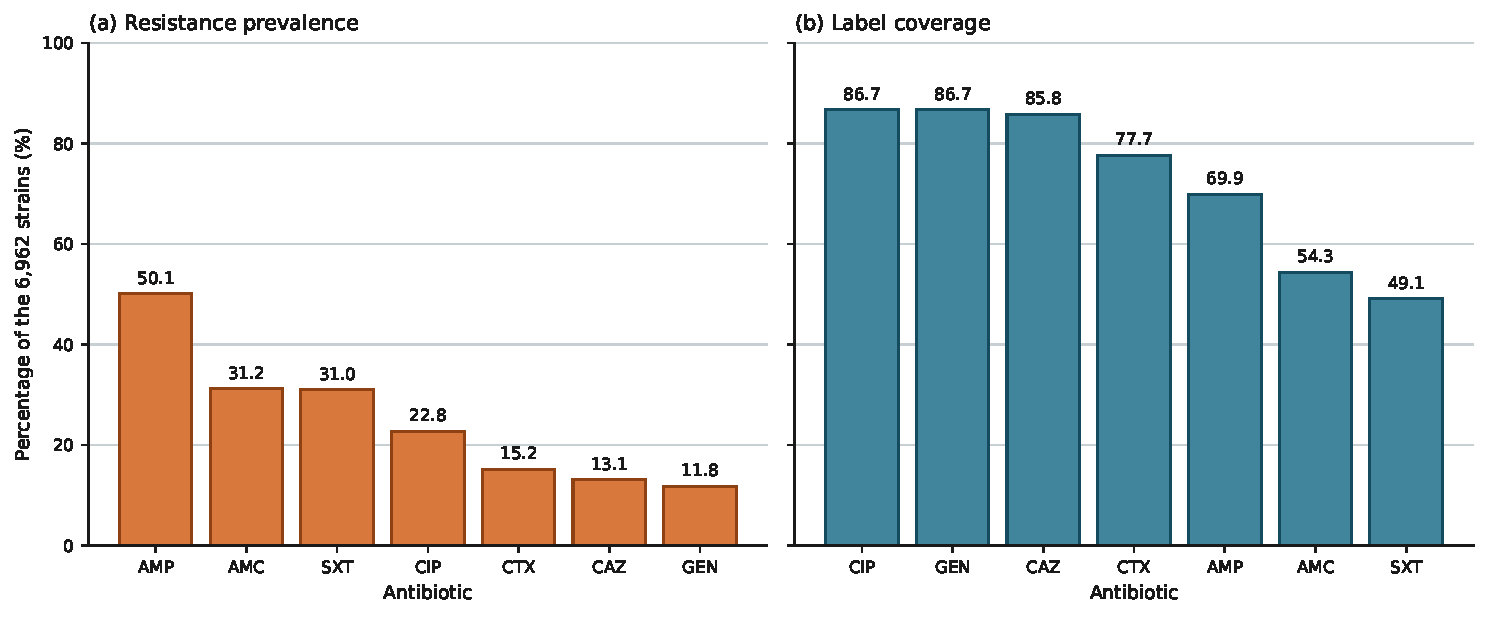
\includegraphics[width=\textwidth]{fig_label_overview.pdf}
\caption{Resistance prevalence and label coverage for the seven retained antibiotics.}
\label{fig:label_overview}
\fignote{\textbf{(a)} Resistance prevalence, ranging from 11.8\% for gentamicin to
50.1\% for ampicillin. \textbf{(b)} Label coverage; no antibiotic carries a label
for more than 86.7\% of the genomes. Both panels share a 0 to 100 per cent axis so
the two quantities can be compared directly.}
\end{figure}


In the cleaned dataset we have built three different genomic views which are complementary to each other, such that the model is not based on one representation. The first is a collection of single-nucleotide polymorphism (SNP) blocks, by gene, of shape $6{,}962 \times 5{,}000 \times 64$, obtained following a two-step gene filter: a variability filter (kept only genes with at least five SNPs), which reduced 18{,}975 genes to 13{,}799, and an importance filter (ranked by gradient-boosting gain), which retained the top 5{,}000 genes. These combined brought 535{,}439 SNPs to 262{,}225, or about 49 percent of the original variants. The second view is a gene presence/absence profile with shape $6{,}962 \times 32{,}441$, which captures resistance genes carried on mobile genetic elements. The third is a collection of shape $6{,}962 \times 5{,}000 \times 4$ per-gene summaries. The filter and all three views are provided in Section~\ref{sec:data}.

The processed data were split into three parts, a training set of 4{,}872 strains, a validation set of 1{,}045 strains and a test set of 1{,}045 strains, about a 70/15/15 split. The lineage holdout below assigns whole groups and so lands on slightly different sizes; Table~\ref{tab:splits} gives the exact figures for all three. The random split randomly assigns strains, thus related strains can be found on both sides. The phylogroup-stratified split preserves an equal distribution of the eight phylogroups in each split. But each phylogroup is present in both the training and test sets. This test, then, does not measure generalisation to unseen lineages but simply the effect of the composition of the lineages. The more challenging question is answered by the sequence-type lineage hold-out split. In this split, any test strain is not of the same sequence type as one of the training strains. All three are described in Section~\ref{sec:comparisons}, including the reason that the phylogroup-stratified split alone was insufficient.

TriLens-MoE-Stack is at the center of the system. It has a feature extractor to extract features from each genomic view and pass them to a separate neural lens. The SNP blocks are fed into a convolutional network called the Motif Pattern Encoder, which identifies small and local mutation patterns in each gene. The gene presence profile goes to the Gene Feature Attention Module, which is a gated-attention network that focuses on the most informative genes. The per-gene statistics are sent to a multi-task head called the Cross-Antibiotic Context Module which provides the ability to share information across similar drugs and helps drugs with fewer labelled examples. The lenses produce a small summary vector and seven per-antibiotic scores.

A Mixture-of-Experts Gating Unit is used to concatenate the three representations into a single 192-length vector. This vector goes through a small network, followed by a softmax. It calculates the weight for each lens individually for each sample and each antibiotic. Consequently, the model is able to use various lenses for a variety of drugs. Simultaneously, the identical gene features feed five base learners, XGBoost on gene features, LightGBM, Random Forest, Logistic Regression, and XGBoost on raw features, each of which makes out-of-fold predictions using five-fold cross-validation. A logistic regression meta-learner combines the neural probability with the five classical probabilities per antibiotic, and a threshold transforms the outcome into a resistant or susceptible call. All the seven antibiotics are forecasted as a multi-label task. The neural lenses are a continuation of a prior GeneAttentionNet precursor that achieved an average precision-recall AUC of approximately 0.769 and supplies the attention signal used later for interpretation.

We present the evaluation using four main pillars. Pillar 1 is concerned with locality. It supports the idea behind the Motif Pattern Encoder. A simple one-dimensional CNN on the entire pan-genome sequence fails the position-shuffling test. This demonstrates that positional locality does not hold across the entire genome. Convolution, however, is more effective within gene blocks. The architecture is Pillar 2. Pillar 3 is interpretability, taken from the model itself through its attention and gating weights and contrasted with post-hoc attribution. The fourth pillar is cross-dataset generalisation, which uses the same methodology on an independent Giessen \textit{E. coli} collection. We are looking for a measure of the success of the system, not only in terms of the correct prediction of resistance, but also one that is appropriate for imbalanced data, primarily precision-recall AUC supported by clinical error rates, so that we will measure how much of the accuracy of the system represents genuine mechanism and how much of it represents population structure.


\FloatBarrier
\section{Preliminary Design and Model Specification}
\label{sec:architecture}

The proposed model TriLens-MoE-Stack is a hybrid architecture in which a stacking meta-learner
is used to join classical machine learning models with neural lenses. The name illustrates the
design: \textit{TriLens} comes from the three genome perspectives the model uses. \textit{MoE} stands
for Mixture of Experts, where a gate determines how much each view should contribute.
\textit{Stack} refers to how the outputs of multiple classical models are combined to produce
the final prediction. The concept is that a bacterial genome can be defined in more
than a single manner and no single definition is complete by itself. A mutation-based view
will miss a resistance gene that arrived on a plasmid, because such a gene is not a mutation at
all. It is simply present, or it is not. A point mutation in a target enzyme is not detectable by the gene presence view. This is
because the gene is present in both resistant and susceptible strains. The only difference is
a single nucleotide change. Instead of selecting between these views, our design incorporates all three and defers to the
model to determine the importance of each view for each antibiotic.


\begin{figure}[H]
  \centering
  \resizebox{0.86\textwidth}{!}{\includestandalone{images/pnn_overall}}
  \caption{Overall dataflow of TriLens-MoE-Stack: three genomic views feed three lenses, which the mixture-of-experts gate fuses before stacking with five classical base learners.}
  \label{fig:trilens-overall}
\end{figure}


This system has three components and the entire architecture is presented in
Figure~\ref{fig:trilens-overall}. To begin with, the three genomic views are processed by a
neural feature extractor that uses three specialised lenses and combines them with a
mixture-of-experts gate. We then use the gene features to train five classical base learners. They make leak-free
out-of-fold predictions. Third, a logistic-regression meta-learner
combines the neural and the classical predictions into a single per-antibiotic prediction.

In the model, each component generates a raw score $z$, whose value may be any real
number, and the score is converted into a probability in the range 0 to 1 with the help of the
logistic sigmoid function,
\begin{equation}
\sigma(z) = \frac{1}{1 + \exp(-z)},
\label{eq:sigmoid}
\end{equation}

\FloatBarrier
\subsection{Rationale for a Hybrid Design Over a Purely Neural One}
\label{subsec:hybrid}

Combining neural and classical models is one of the most crucial design decisions. We use both
instead of one deep neural network. An apparent solution in the contemporary world would be an end-to-end
trained network. We have experimented with that, and it was not very good, but the reason is
in the form of the data, and not in anything wrong with the network. Deep learning works best
in situations where the number of training examples is significantly larger than the number of
input features; our scenario is the opposite with only 6{,}962 labelled strains and hundreds of
thousands of candidate genomic features. The training data can also be memorised in a model that can utilise all this information. Even
with this number of samples, dropout cannot completely avoid that issue.

Gradient boosted trees are much more suited for this type of data. For a feature containing no
signal, the split predictor will just never consider that feature for a split, and it requires
far fewer examples to train a stable model (in this case). The classical arm, then, is not a
fallback or a leftover baseline, it is a load-bearing part of the final design. Meanwhile,
classical models regard each feature as an independent column: they cannot encode the idea
that various mutations near each other within a single gene function as one pattern, nor that
resistance to one cephalosporin says something about another. Those are precisely the types
of tasks a neural network excels at, meaning that the design pairs both, with each arm
addressing the other's weakness. Chapter~\ref{ch:results} provides the proof: on the random
split the neural arm alone hits 0.781 while the combination 0.849, and under the lineage
holdout the classical learners alone score 0.628 while the full model gets 0.634, but the
neural arm yields only 0.472.

\FloatBarrier
\subsection{Classical Base Learners}

The classical arm comprised five base learners: the XGBoost on the gene-aggregated features
(XGB\_gene), LightGBM, Random Forest, Logistic Regression and a second XGBoost on a
chi-squared-prefiltered raw feature matrix (XGB\_raw). These five are trained in an independent
five fold stacking pipeline, and the five out of fold predictions are provided to the
meta-learner of Section~\ref{subsec:metalearner}; the complete configuration is provided with
the hyper-parameters towards the end of this chapter. Each of the five on their own is
presented as a baseline for the proposed model in Chapter~\ref{ch:results}.

Five models might appear to be more than is needed so it is worth explaining why. Only when models of an ensemble commit a variety of errors does the ensemble work. When two
models commit similar errors, their combination does not give much advantage. It averages just
two similar false forecasts. We thus selected five
learners who fail in various manners. Both XGBoost and LightGBM are gradient boosting methods,
but they expand their trees in different ways, thus overfitting to different aspects of the
data. Random Forests use multiple trees, which are averaged and produced to provide a
low-variance but less sharp model. Logistic Regression is also linear and is unable to model
interactions in any way, but it is highly stable. The second XGBoost does not require
gene-level summaries but instead works with raw single-variant features, thus able to capture
signal that is at a single position and would be lost through aggregation. The five are
differentiated between in the three ways that are relevant here: whether a model is able to
pick up combinations of features or only weighs each feature separately, the extent to which
its predictions change when the training data is perturbed slightly, and whether the model
reads the genome one gene at a time or one variant at a time.

Five-fold cross-validation is used to train each base learner, thus each strain is predicted
using a model that was never trained on it. This is more important than it may sound as a
model trained on the full dataset would give overly high scores when asked to make predictions
and the meta-learner would end up putting too much trust in those inflated predictions. This
leak is avoided by out-of-fold prediction, which is why the weights of the stacking layer can
be believed.

\subsubsection{XGBoost}

The gradient boosting idea~\cite{friedman2001gbm} specialised for speed and scale is
XGBoost~\cite{chen2016xgboost} that builds a prediction from multiple shallow decision trees
one by one, each trained from the residual errors of all preceding trees. The process is
illustrated in Figure~\ref{fig:xgboost-workflow}.

\begin{figure}[H]
  \centering
  \makebox[\textwidth][c]{%
    \resizebox{\textwidth}{!}{\begin{tikzpicture}[
  font=\sffamily,
  >={Stealth[length=2.4mm]},
  flow/.style={->,draw=black!70,line width=1.05pt},
  title/.style={font=\bfseries\small,align=center},
  label/.style={font=\scriptsize,align=center,text=black!80},
  panel/.style={rounded corners=2.5pt,line width=.9pt,align=center,
                minimum height=36mm,inner sep=4pt,fill opacity=.45},
  tree/.style={circle,draw=xgbgreen,fill=xgbgreenlight,line width=.8pt,
               minimum size=10mm,inner sep=0pt},
  split/.style={circle,draw=xgbdark,fill=xgbgreen,minimum size=2.2mm,
                inner sep=0pt},
  leaf/.style={circle,draw=xgbdark,fill=white,minimum size=1.7mm,
               inner sep=0pt}
]

\definecolor{xgbblue}{RGB}{33,102,220}
\definecolor{xgbbluelight}{RGB}{223,235,253}
\definecolor{xgborange}{RGB}{235,139,27}
\definecolor{xgborangelight}{RGB}{255,239,215}
\definecolor{xgbgreen}{RGB}{31,168,102}
\definecolor{xgbgreenlight}{RGB}{218,244,231}
\definecolor{xgbdark}{RGB}{20,110,66}
\definecolor{xgbpurple}{RGB}{128,65,180}
\definecolor{xgbpurplelight}{RGB}{239,226,249}
\definecolor{xgbred}{RGB}{211,55,55}

\node[panel,draw=xgbblue,fill=xgbbluelight,minimum width=38mm] (data) {};
\node[title,text=xgbblue!70!black,anchor=north] at ([yshift=-2mm]data.north)
  {Training data};
\begin{scope}[shift={([xshift=-5mm,yshift=7mm]data.center)}]
  \foreach \r in {0,...,4}{
    \foreach \c in {0,...,3}{
      \pgfmathtruncatemacro{\on}{mod(2*\r+\c,3)==0 ? 1 : 0}
      \ifnum\on=1
        \fill[xgbblue] (\c*2.5mm,-\r*2.2mm) rectangle ++(2.5mm,-2.2mm);
      \else
        \fill[white] (\c*2.5mm,-\r*2.2mm) rectangle ++(2.5mm,-2.2mm);
      \fi
    }
  }
  \draw[xgbblue,line width=.35pt] (0,0) grid[xstep=2.5mm,ystep=2.2mm] (10mm,-11mm);
\end{scope}
\node[label,anchor=south] at ([yshift=1mm]data.south)
  {6,962 strains\\$X$: 5,000 genes $\times$ 4 stats\\$y$: R/S label};

\node[panel,draw=xgborange,fill=xgborangelight,minimum width=42mm,
      right=8mm of data] (cv) {};
\node[title,text=xgborange!70!black,anchor=north] at ([yshift=-2mm]cv.north)
  {5-fold CV};
\begin{scope}[shift={([xshift=-10mm,yshift=7mm]cv.center)}]
  \foreach \r in {0,...,4}{
    \foreach \c in {0,...,4}{
      \ifnum\r=\c
        \fill[xgborange] (\c*4mm,-\r*2.5mm) rectangle ++(4mm,-2mm);
      \else
        \fill[xgbgreen!45] (\c*4mm,-\r*2.5mm) rectangle ++(4mm,-2mm);
      \fi
      \draw[white,line width=.25pt] (\c*4mm,-\r*2.5mm) rectangle ++(4mm,-2mm);
    }
  }
\end{scope}
\node[label,anchor=south] at ([yshift=1mm]cv.south)
  {train on 4 folds; predict 1\\\texttt{scale\_pos\_weight}\\$=N_-/N_+$};

\node[panel,draw=xgbgreen,fill=xgbgreenlight,minimum width=76mm,
      right=8mm of cv] (boost) {};
\node[title,text=xgbdark,anchor=north] at ([yshift=-2mm]boost.north)
  {Gradient boosting: 1500 trees};

\node[tree] (t1) at ([xshift=-23mm,yshift=1mm]boost.center) {};
\node[tree] (t2) at ([xshift=-6mm,yshift=1mm]boost.center) {};
\node[font=\small] at ([xshift=9mm,yshift=1mm]boost.center) {$\cdots$};
\node[tree] (tn) at ([xshift=23mm,yshift=1mm]boost.center) {};
\foreach \t in {t1,t2,tn}{
  \node[split] (\t-r) at ([yshift=2.1mm]\t.center) {};
  \node[leaf] (\t-l) at ([xshift=-2.3mm,yshift=-2.2mm]\t.center) {};
  \node[leaf] (\t-q) at ([xshift=2.3mm,yshift=-2.2mm]\t.center) {};
  \draw[xgbdark,line width=.45pt] (\t-r)--(\t-l) (\t-r)--(\t-q);
}
\node[label,below=.7mm of t1] {tree 1};
\node[label,below=.7mm of t2] {tree 2};
\node[label,below=.7mm of tn] {tree 1500};
\node[font=\small,text=xgbdark] at ($(t1)!0.5!(t2)$) {$+$};
\node[font=\small,text=xgbdark] at ($(t2)!0.5!(tn)+(1mm,0)$) {$+$};
\node[label,anchor=south] at ([yshift=1.5mm]boost.south)
  {residual correction; each tree adds $\eta f_t(x)$, $\eta=0.05$};

\node[circle,fill=black!75,text=white,minimum size=10mm,font=\large,
      below=15mm of boost] (sum) {$\sum$};
\node[label,anchor=west] at ([xshift=2mm]sum.east)
  {$F(x)=\sum_t\eta f_t(x)$};

\node[panel,draw=xgbpurple,fill=xgbpurplelight,minimum width=40mm,
      minimum height=28mm,left=10mm of sum] (sig) {};
\node[title,text=xgbpurple,anchor=north] at ([yshift=-2mm]sig.north) {Sigmoid};
\node[font=\small] at ([yshift=-.1cm]sig.center)
  {$\displaystyle \sigma(F)=\frac{1}{1+e^{-F}}$};
\node[label,anchor=south] at ([yshift=-0.02cm]sig.south)
  {convert score\\to probability};

\begin{scope}[shift={([xshift=-60mm,yshift=-2.5mm]sig.west)}]
  \node[font=\normalsize\bfseries,align=center,text=xgbpurple!80!black]
    at (20mm,10.5mm)
    {Out-of-fold resistance probability};
  \shade[left color=xgbgreen,right color=xgbred]
    (0,0) rectangle (40mm,4mm);
  \draw[black!55,line width=.7pt] (0,0) rectangle (40mm,4mm);
  \draw[black!85,line width=1.3pt] (20mm,-1.8mm)--(20mm,6.2mm);
  \node[font=\small,align=center] at (20mm,-4.5mm) {threshold 0.5};
  \node[font=\small,anchor=east] at (-1.5mm,2mm) {0 (S)};
  \node[font=\small,anchor=west] at (41.5mm,2mm) {1 (R)};
  \fill[black] (30mm,2mm) circle (3pt);
  \node[font=\normalsize\bfseries,anchor=south] at (30mm,4mm) {$P=0.71$};
  \coordinate (prob-south-east) at (40mm,0);
  \coordinate (prob-route) at (46mm,-7mm);
\end{scope}

\draw[flow] (data.east)--(cv.west);
\draw[flow] (cv.east)--(boost.west);
\draw[flow] (boost.south)--(sum.north);
\draw[flow] (sum.west)--(sig.east);
\draw[flow] (sig.west)--++(-5mm,0) |- (prob-route) -| (prob-south-east);

\end{tikzpicture}
}%
  }
  \caption{XGBoost base learner: five-fold cross-validation, an additive chain of shrunken trees, then a sigmoid giving the out-of-fold probability.}
  \label{fig:xgboost-workflow}
\end{figure}

Formally, the prediction score for a sample $x$ is the sum of the outputs of $T$ trees:
\begin{equation}
\hat{y}(x) = \sum_{t=1}^{T} \eta\, f_t(x),
\label{eq:xgb_score}
\end{equation}
with each $f_t$ being one tree and $\eta$ being a small learning rate, or shrinkage, which
reduces the contribution of each tree in the model to ensure no one tree is dominant and the
model is enhanced in small, steady steps. Training will reduce a loss that is penalised:
\begin{equation}
\mathcal{L} = \sum_{i=1}^{n} \ell(y_i, \hat{y}_i) + \sum_{t=1}^{T} \Omega(f_t),
\label{eq:xgb_loss}
\end{equation}
and $\ell(\cdot)$ is the binary cross-entropy loss on the $\sigma(\hat{y})$ and $\Omega(f_t)$
is the penalty on trees with a large number of leaves or an excessive number of extreme leaf
values, thus any extra complexity must decrease the error by an amount that justifies its cost.

\vspace{1em}

There are two reasons for XGBoost's inclusion in this list as far as this data is concerned.
If a feature has no information, it is not split, thus a tree can represent a very wide
matrix, and if there is a resistance that requires two mutations together, the tree can split
on one and then the other, which no linear model can do. Where susceptible strains greatly outnumber resistant ones for a drug, the
\texttt{scale\_pos\_weight} parameter is set to the ratio between them. A summary of the genome is represented using XGBoost on the gene-aggregated features, while a
fine-grained view is represented by XGBoost on a chi-squared-prefiltered raw matrix. We choose the number of trees using early stopping~\cite{prechelt1998earlystopping}.

XGBoost also differs from plain gradient boosting in that each tree is fitted using the second
derivative of the loss and not the gradient alone, so a leaf resting on a few strains the model
is already confident about is pulled towards zero. The same quantity sets the bar for splitting:
with $\gamma$ at 0.1, a split that separates two strains but barely moves the loss is never taken.

\subsubsection{LightGBM}

LightGBM~\cite{ke2017lightgbm} applies the same boosting concept with a couple important
shortcuts that are particularly relevant when the data is this wide: histogram binning, which
only uses the bin edges when searching for a split point, and leaf-wise growth, where after
each boosting round it expands whichever single leaf most reduces the error rather than growing
level by level. The outcome is a deeper tree in the areas where the data is
sparse. Growing this way needs a ceiling, or the model keeps splitting one branch until it has
isolated single strains, and ours is \texttt{num\_leaves} at 63 against \texttt{max\_depth} at
6, one short of the 64 leaves a full level-wise tree of that depth would carry. The tree can
therefore spend its budget unevenly without ever growing taller than the XGBoost trees it is
meant to disagree with. The workflow is provided on Figure~\ref{fig:lightgbm-workflow}.

\begin{figure}[H]
    \centering
    \resizebox{0.94\textwidth}{!}{% ============================================================
%  LightGBM base-learner workflow  --  antibiotic resistance prediction.
%  Faithful to the config (stage3_cascadestack_v9, used by the v10 stack):
%  X = 5000 genes x 4 stats, y = R/S, histogram binning, F0 = mu,
%  subsample=0.8, colsample_bytree=0.7, subsample_freq=1,
%  num_leaves=63, max_depth=6, min_child_samples=20, reg_alpha/lambda,
%  eta=0.05, ~1500 trees, early_stopping_rounds=150,
%  sum -> sigmoid -> resistance probability at threshold 0.5.
%  Include with:   \input{images/lightgbm_workflow}   (file goes in images/)
%  Requires in main.tex preamble:
%    \usepackage{amsmath}
%    \usepackage{tikz}
%    \usetikzlibrary{arrows.meta,positioning,fit,backgrounds,calc}
% ============================================================

%% ------------------------------------------------------------------ COLOURS
\definecolor{Cnav}{RGB}{18,52,96}
\definecolor{CnavM}{RGB}{30,80,150}
\definecolor{Cblu}{RGB}{58,140,205}
\definecolor{CbluBG}{RGB}{234,246,253}
\definecolor{CgD}{RGB}{26,110,60}
\definecolor{CgM}{RGB}{45,158,88}
\definecolor{CgL}{RGB}{130,205,148}
\definecolor{Cpur}{RGB}{98,54,176}
\definecolor{CdR}{RGB}{204,52,42}
\definecolor{CdB}{RGB}{32,74,188}
\definecolor{CdG}{RGB}{148,158,168}
\definecolor{Chst}{RGB}{60,124,192}
\definecolor{Cpin}{RGB}{20,110,54}
\definecolor{Csg}{RGB}{0,0,0}

\begingroup
%% Only two text sizes are used anywhere in the figure, so nothing can look
%% "small" next to its neighbours:  \Huge = headline,  \LARGE = all body text.
\renewcommand{\Huge}{\fontsize{41}{48}\selectfont}
\renewcommand{\LARGE}{\fontsize{28}{34}\selectfont}

\begin{tikzpicture}[
  font=\sffamily, x=1cm, y=1cm,
  Aarr/.style={-{Stealth[length=22pt,width=16pt,round]},line width=4.0pt,color=black},
  Garr/.style={-{Stealth[length=22pt,width=16pt,round]},line width=4.0pt,color=CgD},
  Darr/.style={-{Stealth[length=20pt,width=15pt,round]},line width=3.4pt,
                dashed,dash pattern=on 11pt off 7pt,color=CgD},
  Box/.style={draw=CnavM,fill=CbluBG,rounded corners=15pt,line width=3.0pt},
  Sell/.style={draw=CgD,fill=white,circle,line width=3.6pt,minimum size=5.6cm,align=center},
  Iball/.style={draw=#1,fill=#1!13,circle,line width=2.4pt,minimum size=62pt,inner sep=0pt},
  Iball/.default=Cblu,
  Cap/.style={align=center,text=Csg,font=\sffamily\LARGE},
  Hd/.style={align=center,font=\sffamily\LARGE,text=CgD},
  Lbl/.style={font=\sffamily\itshape\LARGE,fill=white,inner sep=7pt},
]

% Recenter: the auto bounding box has extra invisible margin on the left
% (ink sits shifted right relative to the resized/centered figure). Force
% a symmetric box up front so the diagram lines up with the body text
% margins (must come before any node/path is drawn to take effect).
\path[use as bounding box] (-28.9pt,-1250.57532pt) rectangle (1467.31628pt,170.63417pt);

%% ================================================================== TITLE

\node[align=center,font=\sffamily\Huge,text=CnavM] at (23.6,1.7)
  {STAGE 1:\\[2pt]HISTOGRAM-BASED PREPROCESSING};
\node[align=center,font=\sffamily\Huge,text=CnavM] at (44,1.7)
  {STAGE 2:\\[2pt]INITIALISATION};

%% ================================================================== INPUT
\node[Box,minimum width=10.5cm,minimum height=11.4cm] (IB) at (3.5,-6.6) {};
\node[font=\sffamily\Huge,text=CnavM] at (3.5,-2.6) {INPUT DATA};

\node[Iball=Cblu] (Ic1) at (0.9,-4.9) {};
\begin{scope}[shift={(0.9,-4.9)}]
  \draw[Cblu,line width=1.5pt] (-0.32,0.17) to[out=52,in=128] (0.32,0.17);
  \draw[Cblu,line width=1.5pt] (-0.32,-0.17) to[out=-52,in=-128] (0.32,-0.17);
  \foreach \x in {-0.17,0,0.17}{\draw[Cblu,line width=1.3pt] (\x,0.21)--(\x,-0.21);}
\end{scope}
\node[right=10pt of Ic1,text=Cnav,font=\sffamily\LARGE,align=left]
  {Genomic\\[-2pt]Features};

\node[Iball=CnavM] (Ic2) at (0.9,-7.2) {};
\begin{scope}[shift={(0.9,-7.2)},scale=2.3]
  \draw[CnavM,line width=1.5pt,fill=white,rounded corners=1.5pt]
    (-0.13,0.15) rectangle (0.13,-0.15);
  \draw[CnavM,line width=1.5pt,fill=CnavM] (-0.06,0.18) rectangle (0.06,0.13);
  \draw[CnavM,line width=1.1pt] (-0.09,0.06)--(0.09,0.06);
  \draw[CnavM,line width=1.1pt] (-0.09,-0.01)--(0.09,-0.01);
  \draw[CnavM,line width=1.1pt] (-0.09,-0.08)--(0.03,-0.08);
\end{scope}
\node[right=10pt of Ic2,text=Cnav,font=\sffamily\LARGE,align=left]
  {Clinical\\[-2pt]Metadata};

\node[Iball=Cpur] (Ic3) at (0.9,-9.5) {};
\begin{scope}[shift={(0.9,-9.5)}]
  \draw[Cpur,line width=1.5pt] (0,0) circle(0.42);
  \filldraw[Cpur!65] (-0.14,0.13) circle(0.082);
  \filldraw[Cpur!65] ( 0.13,0.09) circle(0.082);
  \filldraw[Cpur!65] (-0.09,-0.14) circle(0.082);
  \filldraw[Cpur!65] ( 0.15,-0.15) circle(0.060);
\end{scope}
\node[right=10pt of Ic3,text=Cnav,font=\sffamily\LARGE,align=left]
  {AMR\\[-2pt]Labels};

\node[font=\sffamily\LARGE,text=CnavM] at (3.5,-11.4) {Training dataset};

%% ================================================================== STAGE 1
\node[Box,minimum width=17cm,minimum height=11.4cm] (S1) at (23.6,-6.6) {};
\begin{scope}[shift={(16.2,-9.2)},xscale=0.70,yscale=0.68]
  \fill[Chst!38] (0.0,0) rectangle (1.0,2.3);
  \fill[Chst!62] (1.2,0) rectangle (2.2,3.9);
  \fill[Chst!88] (2.4,0) rectangle (3.4,5.6);
  \fill[Chst]    (3.6,0) rectangle (4.6,4.5);
  \fill[Chst!68] (4.8,0) rectangle (5.8,2.9);
  \draw[Csg!60,line width=1.8pt,->] (-0.3,0)--(6.6,0);
  \draw[Csg!60,line width=1.8pt,->] (-0.3,0)--(-0.3,6.4);
\end{scope}
\node[anchor=west,align=left,text=Csg,font=\sffamily\LARGE] at (21.0,-6.6)
  {$\bullet$\ Histogram Binning\\
   \quad(continuous $\rightarrow$ discrete)\\[9pt]
   $\bullet$\ Handle Missing Values\\[9pt]
   $\bullet$\ Prepare Feature Values\\[9pt]
   $\bullet$\ Construct Histograms};

%% ================================================================== STAGE 2
\node[Box,minimum width=11cm,minimum height=11.4cm] (S2) at (44,-6.6) {};
\node[draw=Cblu,fill=Cblu,circle,minimum size=4.0cm,font=\Huge,text=white]
  (MU) at (44,-4.2) {$\mu$};
\node[align=center,text=Csg,font=\sffamily\LARGE] at (44,-7.9)
  {Initialise base score with\\the average resistance\\rate in the training data};
\node[draw=CnavM!55,fill=white,rounded corners=10pt,line width=2.2pt,
      font=\Huge,inner sep=11pt] at (44,-10.9) {$F_0=\mu$};

\draw[Aarr] (IB.east) -- (S1.west);
\draw[Aarr] (S1.east) -- (S2.west);

%% ================================================================== STAGE 3 FRAME
\node[draw=CgD,fill=white,rounded corners=22pt,line width=4.4pt,
      fit={(-1.0,-14.6) (49.5,-32.3)}] (S3) {};
\node[font=\sffamily\Huge,text=CgD,fill=white,inner sep=8pt] at (24.25,-14.6)
  {STAGE 3: LEAF-WISE ITERATIVE BOOSTING};
\node[draw=CgD,dashed,dash pattern=on 13pt off 8pt,rounded corners=18pt,
      line width=2.6pt,fit={(0.2,-15.9) (38.9,-29.7)}] (INNER) {};

%% ---- the five steps of one boosting iteration -----------------------------
\node[Sell] (E1) at ( 4.0,-21.9) {};
\node[Sell] (E2) at (11.8,-21.9) {};
\node[Sell] (E3) at (19.6,-21.9) {};
\node[Sell] (E4) at (27.4,-21.9) {};
\node[Sell] (E5) at (35.2,-21.9) {};

\node[Hd] at ( 4.0,-17.5) {1. Gradients\\\& Hessians};
\node[Hd] at (11.8,-17.5) {2. Row + Feature\\Subsampling};
\node[Hd] at (19.6,-17.5) {3. Histogram\\Split Finding};
\node[Hd] at (27.4,-17.5) {4. Leaf-wise\\Tree Growth};
\node[Hd] at (35.2,-17.5) {5. Add Scaled\\Tree Output};

% 1 : gradient / hessian scatter
\begin{scope}[shift={(4.0,-21.9)},scale=1.9]
  \draw[Csg!50,line width=1.1pt,->] (-0.78,0)--(0.84,0);
  \draw[Csg!50,line width=1.1pt,->] (-0.66,-0.78)--(-0.66,0.84);
  \foreach \px/\py in {-0.08/0.38,0.16/0.58,0.40/0.22,-0.36/0.12,0.24/-0.14,
                       -0.12/-0.36,0.48/0.46,-0.46/0.42,0.00/-0.56}
    \filldraw[CdG,fill=CdG!55] (\px,\py) circle(3.6pt);
  \foreach \px/\py in {0.36/-0.48,-0.26/0.58}
    \filldraw[CgD,fill=CgM!70] (\px,\py) circle(3.6pt);
\end{scope}

% 2 : subsampling grid
\begin{scope}[shift={(11.8,-21.9)},scale=1.9]
  \foreach \c in {0,2}{\fill[CdB!22] ({-0.66+\c*0.33},-0.66) rectangle ++(0.33,1.32);}
  \foreach \r in {0,1,3}{\fill[CgM!32] (-0.66,{-0.66+\r*0.33}) rectangle ++(1.32,0.33);}
  \foreach \r in {0,...,3}{\foreach \c in {0,...,3}{
     \draw[CdG!60,line width=0.8pt] ({-0.66+\c*0.33},{-0.66+\r*0.33}) rectangle ++(0.33,0.33);}}
  \draw[Csg!60,line width=1.2pt] (-0.66,-0.66) rectangle (0.66,0.66);
\end{scope}

% 3 : split finding
\begin{scope}[shift={(19.6,-21.9)},scale=1.6]
  \foreach \i/\h in {0/0.42,1/0.72,2/1.14,3/0.78,4/0.48}{
     \fill[CgD!55] ({-0.90+\i*0.36},-0.62) rectangle ++(0.29,\h);}
  \draw[Csg!55,line width=1.2pt] (-0.96,-0.62)--(1.02,-0.62);
  \draw[CdR,line width=2.4pt,dashed] (0.06,-0.80)--(0.06,0.80);
\end{scope}

% 4 : leaf-wise tree
\begin{scope}[shift={(27.4,-21.7)},scale=1.4]
  \draw[CgD,line width=2.2pt]
    (0,0.62)--(-0.56,-0.16) (0,0.62)--(0.56,-0.16)
    (-0.56,-0.16)--(-0.84,-0.94) (-0.56,-0.16)--(-0.28,-0.94)
    (0.56,-0.16)--(0.28,-0.94) (0.56,-0.16)--(0.84,-0.94);
  \filldraw[CgD,fill=CgD] (0,0.62) circle(6.6pt);
  \filldraw[CgD,fill=CgM!80] (-0.56,-0.16) circle(5.8pt);
  \filldraw[CgD,fill=CgM!80] (0.56,-0.16) circle(5.8pt);
  \filldraw[CgM!70,fill=CgL!70](-0.84,-0.94) circle(5.2pt);
  \filldraw[CgM!70,fill=CgL!70](-0.28,-0.94) circle(5.2pt);
  \filldraw[CgM!70,fill=CgL!70](0.28,-0.94) circle(5.2pt);
  \filldraw[CgM!70,fill=CgL!70](0.84,-0.94) circle(5.2pt);
  \node[font=\Huge,text=CgD] at (0,-1.42) {$\cdots$};
\end{scope}

% 5 : scaled tree output
\node[draw=CgD,fill=CgD,circle,minimum size=4.3cm,font=\Huge,text=white]
  at (35.2,-21.9) {$\eta f_t(x)$};

%% ---- captions (every line kept short so columns never collide) ------------
\node[Cap] at ( 4.0,-27.0) {$g_i=\partial L/\partial\hat{y}_i$\\[6pt]
                            $h_i=\partial^2 L/\partial\hat{y}_i^{\,2}$};
\node[Cap] at (11.8,-27.0) {rows: $0.8$\\features: $0.7$};
\node[Cap] at (19.6,-27.0) {scan bin edges\\for maximum\\loss reduction};
\node[Cap] at (27.4,-27.0) {num\_leaves $=63$\\max\_depth $\le 6$\\min\_child $=20$\\L1 + L2 penalty};
\node[Cap] at (35.2,-27.0) {$F_t=F_{t-1}+\eta f_t(x)$\\$\eta=0.05$\\up to $1500$ trees};

%% ---- validation / early stopping -----------------------------------------
\node[Hd] at (44.0,-17.5) {Validation Check\\\& Early Stopping};
\node[draw=CgD,fill=white,dashed,dash pattern=on 12pt off 7pt,rounded corners=16pt,
      line width=3.2pt,minimum width=8.5cm,minimum height=6.0cm] (VB) at (44.0,-21.9) {};
\begin{scope}[shift={(42.4,-22.8)},xscale=0.60,yscale=0.42]
  \fill[CgM!88]  (0.00,0) rectangle (0.90,4.5);
  \fill[CgM!100] (1.20,0) rectangle (2.10,6.2);
  \fill[CgM!80]  (2.40,0) rectangle (3.30,5.0);
  \fill[CgM!60]  (3.60,0) rectangle (4.50,3.2);
  \draw[Csg!48,line width=1.8pt,->] (-0.3,0)--(5.4,0);
  \draw[Csg!48,line width=1.8pt,->] (-0.3,0)--(-0.3,7.4);
\end{scope}
% Nudged right (44.0->44.4) so the bolded "rounds with no gain" line clears
% the dashed inner boosting-loop frame to its left instead of touching it.
\node[Cap] at (44.4,-27.0) {stop after $150$\\rounds with no gain};

%% ---- horizontal flow ------------------------------------------------------
\draw[Garr] (E1) -- (E2);
\draw[Garr] (E2) -- (E3);
\draw[Garr] (E3) -- (E4);
\draw[Garr] (E4) -- (E5);
\draw[Garr] (E5) -- (VB.west);

%% ---- entry from Stage 2 -> Stage 3 (Clean horizontal channel & vertical drop) ----
\draw[Aarr,rounded corners=14pt]
  (S2.south) -- (44.0,-13.2) -- (0.8,-13.2) -- (0.8,-15.9);
\node[Lbl,text=Csg] at (22.4,-13.2) {start the boosting loop from $F_0$};

%% ---- feedback loop        -> enters E1 at 200 deg (lower left) --------------
%% Its vertical run sits at x=-0.4 and stops at y=-22.86, so it can never
%% cross the entry arrow, whose horizontal run is at y=-20.94.
\draw[Darr,rounded corners=12pt]
  (40.0,-24.9) -- (40.0,-31.0) -- (-0.4,-31.0) -- (-0.4,-22.86) -- (E1.200);
\node[Lbl,text=CgD] at (20.0,-31.0) {updated gradients: continue with tree $t+1$};

%% ================================================================== OUTPUT ROW
\node[draw=Cpur,fill=white,rounded corners=16pt,line width=3.0pt,
      minimum width=16.5cm,minimum height=9.4cm] (FB) at (5.5,-39.2) {};
\node[font=\sffamily\LARGE,text=Cpur] at (5.5,-36.1) {FINAL ENSEMBLE MODEL};
\node[align=center,font=\Huge] at (5.5,-39.3)
  {$\displaystyle F(x)=\sum_{t=1}^{T}\eta f_t(x)+\mu$};
\node[Cap] at (5.5,-42.5) {Add initial score $\mu$ to\\the sum of all trees};

\node[draw=Cpur,fill=white,rounded corners=16pt,line width=3.0pt,
      minimum width=18cm,minimum height=9.4cm] (SG) at (24.1,-39.2) {};
\node[font=\sffamily\LARGE,text=Cpur] at (24.1,-36.1) {SIGMOID TRANSFORMATION};
\node[align=center,font=\Huge] at (24.1,-39.3)
  {$\displaystyle P(x)=\sigma\!\left(F(x)\right)=\frac{1}{1+e^{-F(x)}}$};
\node[Cap] at (24.1,-42.5) {Convert raw score to\\resistance probability};

\node[draw=Cpur,fill=white,rounded corners=16pt,line width=3.0pt,
      minimum width=15.5cm,minimum height=9.4cm] (DB) at (41.75,-39.2) {};
\node[font=\sffamily\LARGE,text=Cpur] at (41.75,-36.1) {DECISION (THRESHOLD $=0.5$)};
\begin{scope}[shift={(35.05,-39.6)}]
  \shade[left color=Cpin,right color=Cpur] (0,0) rectangle (13.4,1.2);
  \draw[Csg,line width=1.5pt] (0,0) rectangle (13.4,1.2);
  \draw[white,dashed,line width=2.8pt] (6.7,-0.15)--(6.7,1.35);
  \node[font=\sffamily\LARGE] at (0,1.95) {$0$};
  \node[font=\sffamily\LARGE] at (6.7,1.95) {$0.5$};
  \node[font=\sffamily\LARGE] at (13.4,1.95) {$1$};
\end{scope}
\node[Cap] at (38.35,-42.3) {$P(x)<0.5$\\Susceptible};
\node[Cap] at (45.15,-42.3) {$P(x)\geq0.5$\\Resistant};

%% ---- exit from Stage 3 to the output row ----------------------------------
\draw[Aarr,rounded corners=14pt]
  (VB.east) -- (51.5,-21.9) -- (51.5,-33.3) -- (5.5,-33.3) -- (FB.north);
\node[Lbl,text=Csg] at (28.0,-33.3) {training complete: all $T$ trees are kept};

\draw[Aarr] (FB.east) -- (SG.west);
\draw[Aarr] (SG.east) -- (DB.west);

\end{tikzpicture}
\endgroup}
    \caption{LightGBM workflow: histogram binning, leaf-wise boosting, then the sigmoid
    and the decision at a threshold of $0.5$.}
    \label{fig:lightgbm-workflow}
\end{figure}

Training does not begin from scratch. The initial score $\mu$ is the mean resistance rate of
the training data, and each tree after that is multiplied by a learning rate $\eta$ before it
is added. Due to this, an overall score for a strain will be
\begin{equation}
F(x) = \mu + \sum_{t=1}^{T} \eta\, f_t(x),
\label{eq:lgbm_score}
\end{equation}
Here $\eta = 0.05$ and the raw score is transformed into a probability using
Equation~\eqref{eq:sigmoid}.

\vspace{1em}

The obvious objection is that adding a second gradient boosting model to XGBoost gains nothing.
The two act differently, and are worth keeping. Finally, LightGBM constructs trees in a leaf-wise manner. This enables it to produce extremely imbalanced trees.
Consequently, it is able to pick small and specific patterns that the more balanced trees in
XGBoost do not pick up. As a result, the two make different errors, and that is just what a
stacking ensemble can take advantage of. The hyperparameters used are in
Table~\ref{tab:hyperparameters}.

\subsubsection{Logistic Regression}

The simplest model of the ensemble and the easiest to explain is a Logistic
Regression~\cite{hosmer2013alr}. It assigns a weight value to each feature and then multiplies
the value of each feature by the weight. It then sums all the numbers and feeds it into a
sigmoid to get a probability. There are no trees, feature interactions or hidden layers in the
process. When a mutation is linked to
resistance the weight is positive, when to susceptibility the weight is negative, and the
magnitude of the weight is an indicator of the strength of the effect. The architecture is
shown in Figure~\ref{fig:logistic_regression}.

\begin{figure}[H]
    \centering
    \resizebox{\textwidth}{!}{% !TeX root = ../main.tex
% Works both as a standalone document and as a fragment included by main.tex.
\newif\iflrstandalone
\ifdefined\tikzpicture
  \lrstandalonefalse
  \let\lrenddocument\relax
\else
  \lrstandalonetrue
  \documentclass[tikz,border=15pt]{standalone}
  \usepackage{lmodern}
  \usepackage[T1]{fontenc}
  \usepackage{amsmath,amsfonts}
  \usetikzlibrary{arrows.meta,backgrounds,fit}
  \begin{document}
  \def\lrenddocument{\end{document}}
\fi

\begingroup

% Custom color definitions
\definecolor{cin}{HTML}{BEE3F8}
\definecolor{cexp}{HTML}{FEEBC8}
\definecolor{cgate}{HTML}{E9D8FD}
\definecolor{cattn}{HTML}{C6F6D5}
\definecolor{cout}{HTML}{FED7D7}
\definecolor{cpool}{HTML}{E2E8F0}
\definecolor{cmeta}{HTML}{FBBF24}

\begin{tikzpicture}[
    >=Stealth,
    font=\fontsize{75}{85.5}\selectfont\sffamily,
    text=black,
    node distance=4.2cm and 6.3cm,
    flow/.style={-{Stealth[length=10mm,width=7mm]}, line width=2.4mm, draw=black},
    plain/.style={line width=2.4mm, draw=black},
    circle3d/.style args={#1}{
        circle, draw=#1!65!black, line width=1.2mm,
        fill=#1!42!white,
        preaction={
            draw=#1!65!black, line width=1.2mm,
            fill=#1!55!white,
            transform canvas={xshift=20pt,yshift=20pt}
        }
    },
    input_node/.style={circle3d=cin, minimum size=4.5cm,
        font=\fontsize{75}{85.5}\selectfont\sffamily},
    weight_node/.style={circle3d=cexp, minimum size=4.5cm,
        font=\fontsize{75}{85.5}\selectfont\sffamily},
    sum_node/.style={circle3d=cgate, minimum size=7.8cm, align=center,
        font=\fontsize{87.5}{98}\selectfont\sffamily},
    sigmoid_node/.style={circle3d=cattn, minimum size=9.2cm, align=center,
        font=\fontsize{91.5}{102}\selectfont\sffamily},
    output_node/.style={circle3d=cout, minimum size=7.0cm, align=center,
        font=\fontsize{79}{89.5}\selectfont\sffamily},
    step_node/.style={circle3d=cpool, minimum size=7.0cm, align=center},
    label/.style={font=\fontsize{58.5}{67}\selectfont\sffamily,
        align=center, text width=12cm},
    sub/.style={font=\bfseries\fontsize{68}{68}\selectfont\sffamily, align=center},
    formula/.style={font=\fontsize{85.5}{85.5}\selectfont\sffamily,
        align=center, fill=white, draw=cgate!65!black,
        line width=1.0mm, rounded corners=5mm, inner sep=20pt},
    dots/.style={font=\fontsize{87.5}{98}\selectfont\sffamily},
    layer_box/.style args={#1}{
        fill=#1!14!white, draw=#1!55!black,
        line width=1.2mm, rounded corners=7mm, inner sep=42pt
    }
]

% Recenter: auto bbox has extra invisible margin on the left (input-side
% 3D shadow/box padding), which shifts the visible diagram off the true
% page-margin alignment after resizebox. Force a symmetric box up front
% (must come before any node/path is drawn to take effect).
% ymax extended (689.88 -> 850) to make room for the new headline title
% above the "Error / Loss" node -- xmin/xmax unchanged, so the resizebox
% width-based scale factor (and every font size) is unaffected.
\path[use as bounding box] (-204.99pt,-395pt) rectangle (2208.11525pt,850pt);

% ----------------- HEADLINE TITLE -----------------
% Bold title matching the treatment used above the random-forest.tex
% diagram; placed in the extra headroom created by the bbox extension above.


% ----------------- INPUT LAYER -----------------
\node[input_node] (x0) at (-3.0, 12.0) {$1$};
\node[input_node] (x1) at (-3.0, 6.4) {$x_1$};
\node[input_node] (x2) at (-3.0, 0.7) {$x_2$};
\node[dots] (xd) at (-3.0, -1.7) {$\vdots$};
\node[input_node] (xm) at (-3.0, -6.0) {$x_m$};

\node[label] at (-3.0, 18.0) {Input Layer\\(Features)};
\node[font=\sffamily\fontsize{52}{62}\selectfont,align=center] at (-3.0, -12.0) {($m$ features)};

% ----------------- WEIGHT LAYER -----------------
\node[weight_node] (w0) at (10.0, 12.0) {$w_0$};
\node[weight_node] (w1) at (10.0, 6.4) {$w_1$};
\node[weight_node] (w2) at (10.0, 0.7) {$w_2$};
\node[dots] (wd) at (10.0, -1.7) {$\vdots$};
\node[weight_node] (wm) at (10.0, -6.0) {$w_m$};

\node[label] at (10.0, 18.0) {Weight Layer\\(Parameters)};
\node[font=\sffamily\fontsize{52}{62}\selectfont,align=center] at (10.0, -12.0) {($m+1$ parameters)};

% ----------------- BACKGROUND BOXES -----------------
\begin{scope}[on background layer]
    \node[layer_box=cin, fit=(x0) (xm) (xd)] (input_box) {};
    \node[layer_box=cexp, fit=(w0) (wm) (wd)] (weight_box) {};
\end{scope}

% ----------------- INPUT TO WEIGHT CONNECTIONS -----------------
\draw[plain] (x0) -- (w0);
\draw[plain] (x1) -- (w1);
\draw[plain] (x2) -- (w2);
\draw[plain] (xm) -- (wm);

% ----------------- SUMMATION NODE -----------------
\node[sum_node] (sum) at (24.0, 3.5) {$\displaystyle\sum$};
\node[label] at (24.0, 16.5) {Net Input\\(Linear\\Combination)};
\node[sub] at (24.0, -6.0) {$z = w_0 + \displaystyle\sum_{i=1}^{m} w_i x_i$};

\draw[flow] (w0) -- (sum);
\draw[flow] (w1) -- (sum);
\draw[flow] (w2) -- (sum);
\draw[flow] (wm) -- (sum);

% ----------------- SIGMOID NODE -----------------
\node[sigmoid_node] (sig) at (37.5, 3.5) {$\sigma(z) =$ \\ $\dfrac{1}{1+e^{-z}}$};
\node[label] at (37.5, 14.5) {Sigmoid\\Function};

\draw[flow] (sum) -- node[above, font=\fontsize{58.5}{69}\selectfont\sffamily, yshift=8pt] {$z$} (sig);

% ----------------- OUTPUT NODE -----------------
\node[output_node] (out) at (50.0, 3.5) {$\hat{p}$};
\node[label] at (50.0, 14.5) {Output Layer\\(Probability)};
\node[font=\bfseries\sffamily\fontsize{60}{68}\selectfont,align=center] at (50.0, -6.5) {$\hat{p} = P(y=1\mid x)$};

\draw[flow] (sig) -- (out);

% ----------------- UNIT STEP NODE -----------------
\node[step_node, path picture={
    \draw[line width=2.5mm]
      (path picture bounding box.center) ++(-1.4,-1.0)
      -- ++(1.4,0) -- ++(0,2.0) -- ++(1.4,0);
}] (step) at (61.5, 3.5) {};
\node[label] at (61.5, 14.5) {Unit Step\\(Prediction)};
\node[font=\bfseries\sffamily\fontsize{60}{68}\selectfont,align=center] at (61.5, -10.0) {$\hat{y} = \mathbf{1}(\hat{p} \geq \tau)$};

\draw[flow] (out) -- (step);

% ----------------- FINAL PREDICTION -----------------
\coordinate (final_out) at (70.0, 3.5);
\draw[flow] (step) -- (final_out)
    node[right, font=\fontsize{67}{75}\selectfont\sffamily, align=center]
    {$\hat{y}$\\(0 or 1)};

% ----------------- ERROR / LOSS FEEDBACK -----------------
\node[draw=cmeta!65!black, dashed, rounded corners=6mm, line width=1.4mm,
      font=\fontsize{68}{76}\selectfont\sffamily,
      fill=cmeta!42!white, inner sep=28pt,
      preaction={
          draw=cmeta!65!black, dashed, rounded corners=6mm, line width=1.4mm,
          fill=cmeta!55!white,
          transform canvas={xshift=20pt,yshift=20pt}
      }] (loss) at (37.5, 22.0) {Error / Loss};

% Feedback loop
\coordinate (feedback_start) at (68.5, 3.5);

\draw[dashed, line width=2.0mm] (feedback_start) -- (68.5,22.0);
\draw[dashed, line width=2.0mm] (68.5,22.0) -- (loss.east);

\coordinate (feedback_turn) at (17.0,22.0);
\draw[dashed, flow] (loss.west) -- (feedback_turn) |-
    (weight_box.north east);

\end{tikzpicture}

\endgroup
\lrenddocument}
    \caption{Logistic Regression: a weighted sum of the inputs passed through a sigmoid.}
    \label{fig:logistic_regression}
\end{figure}

In the model, the features are linearized to give a score,
\begin{equation}
z = w^\top x + b,
\label{eq:logreg_score}
\end{equation}
where $w$ is the weight of the features and $b$ is a bias that changes the aggregate baseline
and the score is transformed to a probability using Equation~\eqref{eq:sigmoid}. Training is
used to minimise penalised binary cross-entropy loss,
\begin{equation}
\mathcal{L} = -\frac{1}{n}\sum_{i=1}^{n}\left[y_i \log p_i + (1-y_i)\log(1-p_i)\right] + \lambda\,R(w),
\label{eq:logreg_loss}
\end{equation}
with the first term preferring to penalise certain confident errors more than uncertain ones,
and the second term, $R(w)$, ensures that the weights are kept small in order to prevent any
single feature dominating.

Its value to the ensemble lies in that simplicity. Since it cannot represent interactions, it cannot invent
interactions, and consequently overfits much less than the tree ensembles: when the boosting
models become over-confident on a given strain the linear model remains closer to the average
and the meta-learner can learn on it.

\subsubsection{Random Forest}

Random Forest~\cite{breiman2001rf} operates in the reverse direction to boosting: a large
number of trees are constructed and averaged, not in series. Two sources of randomness ensure
that they are not duplicates of each other, a bootstrap sample of the
strains~\cite{breiman1996bagging} per tree and random selection of features to be explored at
each split, making their respective errors point in different directions and most of them
cancel. The architecture is shown in Figure~\ref{fig:random_forest_architecture}.

\begin{figure}[H]
    \centering
    \begin{adjustbox}{max width=\textwidth, max totalheight=0.60\textheight, center}
    
\newcommand{\rfdrawtree}[3]{
  \begin{scope}[shift={(#2,#3)}]
    \node[treenode] (root-#1) at (0,0) {};
    \node[treenode] (l1-#1)   at (-1.4,-1.0) {};
    \node[treenode] (r1-#1)   at (1.4,-1.0) {};
    \node[treenode] (ll1-#1)  at (-2.1,-2.0) {};
    \node[treenode] (ll2-#1)  at (-0.7,-2.0) {};
    \node[treenode] (rr1-#1)  at (0.7,-2.0) {};
    \node[treenode] (rr2-#1)  at (2.1,-2.0) {};

    \node[treenodew] (lll1-#1) at (-2.6,-3.2) {};
    \node[treenodew] (lll2-#1) at (-1.7,-3.2) {};
    \node[treenodew] (ll21-#1) at (-1.0,-3.2) {};
    \node[treenodew] (ll22-#1) at (-0.3,-3.2) {};
    \node[treenodew] (rr11-#1) at (0.3,-3.2) {};
    \node[treenodew] (rr12-#1) at (1.0,-3.2) {};
    \node[treenodew] (rr21-#1) at (1.7,-3.2) {};
    \node[treenodew] (rr22-#1) at (2.6,-3.2) {};

    \draw[line] (root-#1) -- (l1-#1);   \draw[line] (root-#1) -- (r1-#1);
    \draw[line] (l1-#1) -- (ll1-#1);    \draw[line] (l1-#1) -- (ll2-#1);
    \draw[line] (r1-#1) -- (rr1-#1);    \draw[line] (r1-#1) -- (rr2-#1);
    \draw[line] (ll1-#1) -- (lll1-#1);  \draw[line] (ll1-#1) -- (lll2-#1);
    \draw[line] (ll2-#1) -- (ll21-#1);  \draw[line] (ll2-#1) -- (ll22-#1);
    \draw[line] (rr1-#1) -- (rr11-#1);  \draw[line] (rr1-#1) -- (rr12-#1);
    \draw[line] (rr2-#1) -- (rr21-#1);  \draw[line] (rr2-#1) -- (rr22-#1);
  \end{scope}

  \draw[ar] (ds#1.south) -- (root-#1.north);

  \node[box, minimum width=5.2cm, mainfont]
    (t#1lbl) at (#2,#3-5.3) {Decision\\Tree #1};
  \draw[line] (#2,#3-3.4) -- (t#1lbl.north);
}

\begin{tikzpicture}[
    >=Stealth,
    font=\bfseries\fontsize{24}{26.5}\selectfont\sffamily,
    mainfont/.style={font=\bfseries\fontsize{24}{26.5}\selectfont\sffamily},
    titlefont/.style={font=\bfseries\fontsize{27}{29.5}\selectfont\sffamily},
    notefont/.style={font=\itshape\fontsize{19}{21}\selectfont\sffamily},
    ar/.style={-{Stealth[length=5.5mm,width=4.0mm]}, line width=1.2mm, draw=black},
    treeflow/.style={-{Stealth[length=5.5mm,width=4.0mm]}, line width=1.2mm,
        draw=black, shorten <=3pt, shorten >=3pt},
    line/.style={line width=1.2mm, draw=black},
    prism/.style args={#1}{
        rectangle, draw=#1!65!black, line width=0.5mm,
        fill=#1!42!white, align=center, minimum height=2.4cm, inner sep=18pt,
        append after command={
            \pgfextra{
                \begin{pgfonlayer}{background}
                \filldraw[fill=#1!27!white, draw=#1!65!black, line width=0.5mm]
                    (\tikzlastnode.north west) --
                    ([xshift=12pt,yshift=12pt]\tikzlastnode.north west) --
                    ([xshift=12pt,yshift=12pt]\tikzlastnode.north east) --
                    (\tikzlastnode.north east) -- cycle;
                \filldraw[fill=#1!55!white, draw=#1!65!black, line width=0.5mm]
                    (\tikzlastnode.north east) --
                    ([xshift=12pt,yshift=12pt]\tikzlastnode.north east) --
                    ([xshift=12pt,yshift=12pt]\tikzlastnode.south east) --
                    (\tikzlastnode.south east) -- cycle;
                \end{pgfonlayer}
            }
        }
    },
    box/.style={prism=cexp},
    graybox/.style={prism=cin},
    outbox/.style={prism=cgate},
    finalbox/.style={prism=cout},
    predbox/.style={rectangle, rounded corners=3mm, draw=black,
        line width=1.0mm, fill=white, minimum width=5.8cm,
        minimum height=1.8cm, align=center, mainfont},
    treenode/.style={circle, draw=black, line width=0.9mm,
        fill=cexp, fill opacity=0.85, minimum size=22pt, inner sep=0pt},
    treenodew/.style={circle, draw=black, line width=0.9mm,
        fill=cin, fill opacity=0.65, minimum size=22pt, inner sep=0pt},
    lbl/.style={notefont}
]

\node[graybox, minimum width=7.0cm, mainfont]
    (input) at (0,2.5) {Training Data};

\def\dsY{-2.8}
\node[graybox, minimum width=6.2cm, inner xsep=10pt, mainfont,
      font=\bfseries\fontsize{20}{22.5}\selectfont\sffamily] (ds1) at (-16.0,\dsY)
    {BOOTSTRAP\\SAMPLE 1};
\node[graybox, minimum width=6.2cm, inner xsep=10pt, mainfont,
      font=\bfseries\fontsize{20}{22.5}\selectfont\sffamily] (ds2) at (-5.3,\dsY)
    {BOOTSTRAP\\SAMPLE 2};
\node[graybox, minimum width=6.2cm, inner xsep=10pt, mainfont,
      font=\bfseries\fontsize{20}{22.5}\selectfont\sffamily] (dsd) at (5.3,\dsY)
    {$\boldsymbol{\cdots}$};
\node[graybox, minimum width=6.2cm, inner xsep=10pt, mainfont,
      font=\bfseries\fontsize{20}{22.5}\selectfont\sffamily] (dsN) at (16.0,\dsY)
    {BOOTSTRAP\\SAMPLE $N$};

\coordinate (sampleRail) at (0,0.0);
\draw[line] (input.south) -- (sampleRail);
\draw[line] (ds1.north |- sampleRail) -- (dsN.north |- sampleRail);
\foreach \sample in {ds1,ds2,dsd,dsN}{
    \draw[ar] (\sample.north |- sampleRail) -- (\sample.north);
}

\node[lbl, align=center, fill=white, inner sep=10pt, draw=black,
      line width=0.5mm, rounded corners=2mm] at (0,-5.5)
    {Independent trees use a random subset of features at each split};

\def\treeY{-7.0}
\rfdrawtree{1}{-16.0}{\treeY}
\rfdrawtree{2}{-5.3}{\treeY}
\node[titlefont, scale=1.6] at (5.3,\treeY-1.6) {$\cdots$};
\rfdrawtree{N}{16.0}{\treeY}
\node[titlefont, scale=1.6, text=black!55] at (5.3,\treeY-5.3) {$\cdots$};

\node[predbox] (pred1) at (-16.0,-14.8) {Prediction 1};
\node[predbox] (pred2) at (-5.3,-14.8) {Prediction 2};
\node[predbox] (predN) at (16.0,-14.8) {Prediction $N$};
\node[titlefont, scale=1.6, text=black!55] at (5.3,-14.8) {$\cdots$};

\draw[treeflow] (t1lbl.south) -- (pred1.north);
\draw[treeflow] (t2lbl.south) -- (pred2.north);
\draw[treeflow] (tNlbl.south) -- (predN.north);

\node[prism=cgate, minimum width=11.0cm, minimum height=2.6cm,
      mainfont]
    (vote) at (0,-18.8) {Combine Predictions};

\coordinate (predictionRail) at (0,-16.5);
\draw[line] (pred1.south) -- (pred1.south |- predictionRail);
\draw[line] (pred2.south) -- (pred2.south |- predictionRail);
\draw[line] (predN.south) -- (predN.south |- predictionRail);
\draw[line]
    (pred1.south |- predictionRail) -- (predN.south |- predictionRail);
\draw[ar] (predictionRail) -- (vote.north);

\node[outbox, minimum width=12.0cm, minimum height=2.8cm,
      mainfont]
    (agg) at (0,-22.5) {Majority Vote\\or Probability Average};
\draw[ar] (vote.south) -- (agg.north);

\node[finalbox, minimum width=10.5cm, minimum height=2.8cm,
      mainfont]
    (out) at (0,-26.3) {Final Prediction\\Resistant / Susceptible};
\draw[ar] (agg.south) -- (out.north);

\end{tikzpicture}
    \end{adjustbox}
    \caption{Random Forest: independent trees trained on bootstrapped samples, then averaged.}
    \label{fig:random_forest_architecture}
\end{figure}

Given a sample $x$, the predicted probability of resistance is the average of the per-tree
probability estimates:
\begin{equation}
\hat{p}(x) = \frac{1}{T} \sum_{t=1}^{T} p_t(x),
\label{eq:rf_score}
\end{equation}
where $p_t(x)$ is the proportion of the leaf in the tree $t$ that $x$ visits that is of class
one. Graded probabilities are meta-features that would not be provided by a hard majority
vote, and are required by the stacking layer.

\vspace{1em}

Random Forest adds stability instead of optimum accuracy. The predictions are relatively
robust to slight changes in the training data, which is a property that boosting models in
general do not have, and thus the ensemble will certainly possess an element that is hard to
push to one extreme.

\FloatBarrier
\subsection{Neural Lenses}

The neural feature extractor has three lenses that correspond to the three genomic views.
Each reads its respective view, creates a short representation in a 64-length summary vector
$z$, and outputs seven scores, for each antibiotic. All three struggle with the same
challenge: each strain is characterised by thousands of genes, but most of those genes
are not relevant for any one antibiotic and which ones are relevant changes with drug. This
calls for a mechanism that can focus on a handful of pertinent genes without any prior
knowledge as to which. This mechanism is the gated attention of Ilse et\
al.~\cite{ilse2018attention}, which is an extension of the attention
mechanism~\cite{vaswani2017attention} for the scenario where only a few items in a large bag
are informative. Every element $h$ is given a relevance score,
\begin{equation}
e = w^\top \big(\tanh(V h) \odot \sigma(U h)\big),
\label{eq:gated_attn}
\end{equation}
and the $U$, $V$ and $w$ are learned in training and $\odot$ represents element-wise
multiplication. The expression has two branches for a reason. The $\tanh$ branch puts forward
the degree to which this element appears to be valuable and results in a value between $-1$
and $1$. The $\sigma$ branch is a gate which generates a value in the range 0 to 1 that
determines the portion of that proposal to permit through. An element may thus be suppressed
even though it may appear on the surface to be informative which cannot be done by ordinary
attention. The scores are normalised with a softmax giving them weights which sum up to one
and the pooled summary is the weighted sum of the elements. In short, each lens becomes the sole author of the very brief write-up of a lengthy document.

\subsubsection{Motif Pattern Encoder}

The Motif Pattern Encoder reads SNP blocks, whose shape is $(G, L)$ where $G = 5{,}000$ genes
and $L = 64$ positions per gene. It is used to identify short local motifs, or patterns, of
mutations within a gene. The reasoning is that one mutation is generally silent, but then two or three mutations in
the same gene, close together in the DNA, are more likely to break or change the protein that
the gene codes for.
The natural device to this is a convolutional network, since a convolution is performed by
sliding a small window over a sequence and finding a pattern anywhere in the sequence.

Each gene has two convolutional layers stacked:
\begin{equation}
h_g = \mathrm{ReLU}\!\left(\mathrm{Conv1d}_{16 \to 32}\big(\mathrm{ReLU}(\mathrm{Conv1d}_{1 \to 16}(x_g))\big)\right),
\label{eq:expertA_conv}
\end{equation}
with windows of width three, with dropout~\cite{srivastava2014dropout} between layers. The
initial layer is trained on 16 simple patterns and the second layer is trained on 32 more
complex patterns based on the simple ones, thus, the model is constructed to be based on
simple motifs and then compound motifs. A masked max-pooling step then prunes each gene to a
fixed length vector by retaining, in each learned pattern, the strongest response it could
find anywhere in that gene. The mask makes sure that padding positions in shorter genes are
not considered as real data. The per-gene vectors are lastly pooled between genes with the
gated attention of Equation~\eqref{eq:gated_attn} to yield the representation
$z_A \in \mathbb{R}^{64}$ and per-antibiotic scores $\ell_A \in \mathbb{R}^{7}$.
Figure~\ref{fig:expertA} shows the encoder.

\begin{figure}[H]
  \centering
  \resizebox{\textwidth}{!}{\includestandalone{images/pnn_expertA}}
  \caption{Motif Pattern Encoder: a SNP block passes through two convolutional layers, masked max-pooling, and gated attention over genes.}
  \label{fig:expertA}
\end{figure}

This design is based on a direct experiment as opposed to reasoning solely. When a
convolution is done, only near positions in the input actually are related which is called
locality. We checked that this assumption is true throughout the entire pan-genome by
training a plain one-dimensional convolutional network on the full sequence of variants,
\begin{equation}
h^{(l)} = \mathrm{MaxPool}\!\left(\mathrm{ReLU}\!\left(\mathrm{BN}\!\left(\mathrm{Conv1d}_l\!\left(h^{(l-1)}\right)\right)\right)\right),
\qquad l = 1, 2, 3,
\label{eq:naive_cnn}
\end{equation}
with $h^{(0)}$ the embedded variant sequence and four convolutional layers of widths 9, 7, 5
and 3 and channel sizes 64, 96, 128 and 128 in turn, the last of which skips the pooling step
and is instead reduced by global average pooling and a single linear readout,
$\hat{\ell} = w^\top \mathrm{AvgPool}(h^{(4)}) + b$, and then randomly shuffling the order
of the variants. If position were actually meaningful, then shuffling would have hurt performance but it did
not: the model performed equally well with the shuffled input, providing further evidence that
the order of variants in the pan-genome has no signal and that a convolution at this scale is
learning nothing about position. Within a single gene this is not the case, since there the
order of sequence is biologically real. The Motif Pattern Encoder thus only uses convolution
within blocks of genes, which is precisely where the locality assumption passes the test.
Pillar 1 is this experiment, and the results are presented in Chapter~\ref{ch:results}.

\subsubsection{Gene Feature Attention Module}
\label{subsec:lensB}

The Gene Feature Attention Module reads the presence and absence profile of the genes, a
binary vector of 32{,}441 genes indicating which genes each strain has. It has been employed to
detect acquired resistance, but in a totally different manner than is required for setting up
a system to detect mutational resistance. The mechanism by which a strain can become resistant is by acquiring a
completely new gene, the original strain did not have, usually through a plasmid. This gene
is either missing or there it is; so there is no amount of mutation analysis that would find
it. The reason why this view is present is to make such a case.

It assigns each gene a learnable embedding, which is just a short vector that the model
learns that represents what that gene actually means. This embedding is only permitted to
have an effect if the gene is contained in that strain,
\begin{equation}
\tilde{e}_k = x_k \, E_k, \qquad k = 1, \dots, G_{\mathrm{pa}},
\label{eq:expertB_embed}
\end{equation}
where $E_k \in \mathbb{R}^{d_{\mathrm{token}}}$ is the learned embedding of gene $k$, and
$x_k \in \{0,1\}$ indicates whether the strain possesses gene $k$. When $x_k = 0$
$\tilde{e}_k$ is the zero vector, and therefore a missing gene cannot affect the prediction at
all regardless of what its embedding has learned. Genes that are absent in a strain are also
masked out by setting their attention scores to $-\infty$ just before the softmax of
Equation~\eqref{eq:gated_attn}, which pushes their weight to exactly zero and redundantly
provides the same conclusion.

\vspace{1em}

We cannot apply Equation~\eqref{eq:gated_attn} to $\tilde{e}_k$ directly and this is the only
point in the design we alter the mechanism, but not the data it accesses. Gated attention
scores every item based on the item representation. But for any gene the strain carries, this
representation is $\tilde{e}_k = E_k$, which is the same vector for each strain. The score
would be the same for each strain, too, the softmax would just renormalise based on which
genes that strain just happens to have, and the lens would collapse to a global gene ranking
based on presence. It was unable to convey the message that a certain gene is important to a
certain isolate, which is the whole point of laying focus here. This is not the case with the
other two lenses, as the inputs of these lenses already vary depending on the strain.

\vspace{1em}

The score is therefore dependent on the strain. For the remainder of the research, we will refer
to this as \emph{strain conditioning}. We ablate it against the standard method in
Section~\ref{subsec:attnfix}.

\begin{equation}
c = \frac{1}{\max(n_b, 1)} \sum_{k=1}^{G_{\mathrm{pa}}} \tilde{e}_k,
\qquad n_b = \sum_k x_k,
\label{eq:expertB_ctx}
\end{equation}

Here $c$ is the average embedding of the genes this strain really carries, and each gene is
scored in the company it maintains,

\begin{equation}
s_k = w^\top\Big(\tanh\big(V \tilde{e}_k + V_c\, c\big) \odot
\sigma\big(U \tilde{e}_k + U_c\, c\big)\Big),
\label{eq:expertB_score}
\end{equation}

with $V_c$ and $U_c$ being added projections. A sum of two projections is the same as a single
projection on the concatenation $[\tilde{e}_k;\, c]$, but is useful because it broadcasts $c$
rather than realising a tensor of size $B \times 32{,}441 \times 2 d_{\mathrm{token}}$, a size
that would be unaffordable at this number of genes. The additional cost is two
$d_{\mathrm{token}} \times d_{\mathrm{attn}}$ matrices. An ablation study comparing this term with the
baseline method can be found in Section~\ref{subsec:attnfix}. It increases the neural lenses by
0.035 average PR-AUC under the lineage holdout. The attention weights also modify the genes
that are being selected. The attended genes, in turn, contain 41\% as much resistance
information as the genes selected by SHAP when it is not present. They have 89\% as much
with it.

\vspace{1em}

The attention calculation is performed at single precision as opposed to half precision, as
accumulating the sum over 32{,}441 genes at reduced precision adds sufficient round-off error
to disrupt training. The attended embeddings are pooled and projected,
\begin{equation}
z_B^{\mathrm{pre}} = \sum_{k=1}^{G_{\mathrm{pa}}} a_k\, \tilde{e}_k,
\qquad
z_B = \mathrm{GELU}\!\left(W_B\, z_B^{\mathrm{pre}} + b_B\right) \in \mathbb{R}^{64},
\label{eq:expertB_out}
\end{equation}
with per-antibiotic scores $\ell_B \in \mathbb{R}^{7}$ read off $z_B$ by seven independent
linear heads, as illustrated in Figure~\ref{fig:expertB}.

\begin{figure}[H]
  \centering
  \resizebox{\textwidth}{!}{\includestandalone{images/pnn_expertB}}
  \caption{Gene Feature Attention Module: the gene presence and absence profile is embedded and pooled with masked attention over the present genes.}
  \label{fig:expertB}
\end{figure}

In a fully connected layer, each unit would require tens of thousands of weights (one per
input), and with a total of only 6{,}962 training samples, a layer that large would overfit
almost without fail. This is avoided by attention which does not increase the number of parameters as
the number of genes increases, the same small scoring function is used on each gene
separately. It also provides us with something that a dense layer does not: the weights of
attention are readable, and we can query which genes the model focused on to make a
particular prediction. The interpretability analysis of Pillar 3 is based on that readout.

\subsubsection{Cross-Antibiotic Context Module}

The Cross-Antibiotic Context Module reads the per-gene summary statistics, of shape $(G, 4)$,
where each gene is characterised (not by its complete mutation pattern) by four numbers. It
does not have the same purpose as the other two lenses: rather than deriving a new type of
signal out of the genome, it takes advantage of the interactions among the antibiotics
themselves. The rationale is biological. Drug resistance to two drugs of the same class is
normally caused by the same mechanism. If a strain develops an enzyme that can hydrolyse cefotaxime, it is likely that it will also
hydrolyse ceftazidime, as both are cephalosporins and the enzyme will act on both. In the event that we train seven absolutely independent
models, each drug must learn its own mechanism using its own labels, and the drugs that have
few resistant samples do not get enough chances to learn anything reliable. When two or more drugs within a drug class have a common representation, evidence from a
well-represented drug can assist the model with a poorly-represented drug in the same class. Figure~\ref{fig:coresistance} also puts that
argument to the test of our own data, and the answer to it is not wholly the one which the
biology predicts. That is the shared-mechanism account exactly: the two cephalosporins are by
far the most closely associated pair, at $\phi = 0.84$, and nothing else even remotely
approaches that. But below it, membership in the classes ceases to be a useful predictor.
Ampicillin is associated with trimethoprim-sulfamethoxazole at 0.55, in two unrelated classes,
about as strongly as it is with amoxicillin-clavulanate at 0.54 within its own; and ciprofloxacin,
which has no second member in the present case, is at 0.51 and 0.52 with the two
cephalosporins. Resistance genes on the same plasmid or integron travel together, regardless of whether they
target the same drug, and this group shows both patterns at once. The figure also shows why
small overlap values here cannot be used as a ranking: some antibiotic pairs are measured
against only 235 strains (amoxicillin-clavulanate and trimethoprim-sulfamethoxazole), while
others are measured against 6{,}030 (ciprofloxacin and gentamicin), so the values are not
directly comparable.

This influences the design that ensues. The cephalosporin connection would be detected by a
module that exchanged information solely inside classes (and not between them), and it would
fail to learn any cross-class link, which explains why the class-specific heads below are
initially succeeded by a refinement step that is free to learn connections not present in the
hierarchy.

\begin{figure}[htb]
  \centering
  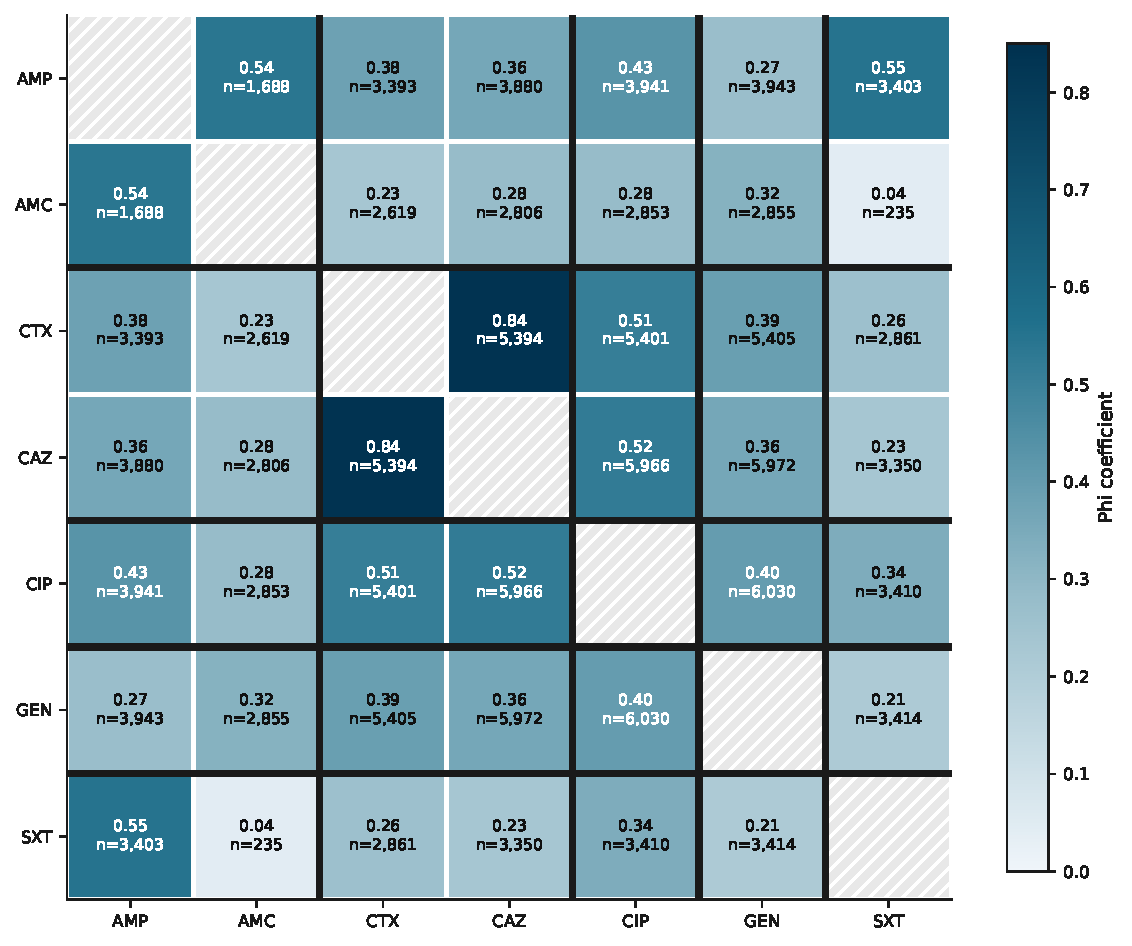
\includegraphics[width=\textwidth]{fig_coresistance.pdf}
  \caption{Pairwise co-resistance ($\phi$) between antibiotics.}
  \label{fig:coresistance}
  \fignote{Each cell is computed on the strains labelled for both drugs ($n$ shown).
  The heavy rules separate the drug classes: penicillins (AMP, AMC), cephalosporins
  (CTX, CAZ), the fluoroquinolone (CIP), the aminoglycoside (GEN) and the
  folate-pathway inhibitor (SXT). The diagonal is hatched because a drug has no
  co-resistance with itself.}
\end{figure}

This is implemented directly in the Cross-Antibiotic Context Module. Each gene's four
statistics are first transformed by a small multilayer perceptron (one per gene); then, for
global pooling across genes, gated attention is used to compute $z_C \in \mathbb{R}^{64}$.
This common representation is then decoupled into one distinct projection for each drug class;
the penicillins (AMP, AMC), the cephalosporins (CTX, CAZ), the fluoroquinolone (CIP), the
aminoglycoside (GEN), and the folate-pathway inhibitor (SXT). All of the data prior to this
split is learned jointly from all seven drugs; all of the data after this is specific to one
class,
\begin{equation}
t = \mathrm{GELU}(W_t z_C + b_t) \in \mathbb{R}^{32},
\qquad
u_g = \mathrm{GELU}(W_g t + b_g) \in \mathbb{R}^{16},
\label{eq:expertC_trunk}
\end{equation}
where $t$ is the shared trunk output and $u_g$ is the projection for drug class
$g \in \{\text{penicillin}, \text{cephalosporin}, \text{fluoroquinolone}, \text{aminoglycoside},
\text{folate}\}$. Now each antibiotic reads its initial score, according to the projection of
its own class only,
\begin{equation}
\ell^{\mathrm{init}}_{C,a} = w_a^\top u_{g(a)} + b_a,
\label{eq:expertC_ablogit}
\end{equation}
where $g(a)$ is the drug class antibiotic $a$ belongs to. Lastly, a co-resistance refinement step allows the prediction for one antibiotic to modulate
the prediction for a related one,
\begin{equation}
r = \mathrm{MLP}\!\left(\left[z_C \, ; \, \ell^{\mathrm{init}}_{C}\right]\right) \in \mathbb{R}^{7},
\qquad
\ell_C = \ell^{\mathrm{init}}_{C} + \alpha\, r,
\label{eq:expertC_cores}
\end{equation}
with $\alpha$ a learned scalar starting with a value of 0.1. This step is initialised to close
to zero, such that the model initially ignores it, and only considers it when the data
supports the step which ensures that a spurious relationship between two drugs is not baked
in at the beginning. Figure~\ref{fig:expertC} shows that $\ell_C$ is produced by the lens in
$\mathbb{R}^{7}$.

\begin{figure}[H]
  \centering
  \resizebox{\textwidth}{!}{\includestandalone{images/pnn_expertC}}
  \caption{Cross-Antibiotic Context Module: per-gene statistics are transformed, pooled with attention, and passed through drug-class heads with co-resistance refinement.}
  \label{fig:expertC}
\end{figure}

It is easier to train seven separate models and this is how we started. The issue is the lack
of balance in drugs. The number of resistant strains of gentamicin is low compared to
ampicillin and therefore there is nothing much to learn by a gentamicin-only model. There is a common base shared across all antibiotics. This base learns from the labels of
every drug, not just one. This is exactly what multi-task learning is designed to do.
Nonetheless, if the common base acquires a misleading pattern, it influences all drugs. To
limit this problem, there is a branch for each drug. Some of those mistakes can still be
corrected by these branches.

\FloatBarrier
\subsection{Mixture-of-Experts Gating and Representation Fusion}
\label{subsec:moegate}

When each of three lenses has made an opinion about each of the seven antibiotics, their
opinions will not necessarily be consistent, and here the question is to what to do with
them. The easiest would be to average the three. We discarded that, since averaging supposes
that all the three lenses will be equally useful, and they are not. When the resistance of a
drug is due to an acquired plasmid gene, the Gene Feature Attention Module should prevail and
the Motif Pattern Encoder can do practically nothing with it. In the case of a drug whose
resistance is due to a point mutation in a target enzyme, the opposite holds true. A decision based on the
average would drown out the voice of a stronger lens (and its view) with two weaker ones.

The mixture-of-experts gate~\cite{jacobs1991moe, shazeer2017moe} addresses this by learning
weights, rather than fixing them, and by learning them individually, one strain at a time, and
each antibiotic at a time. The three representations are combined into a single vector
$z = [z_A; z_B; z_C] \in \mathbb{R}^{192}$ and fed through a small network and softmax to
obtain
\begin{equation}
g = \mathrm{softmax}\big(\mathrm{MLP}([z_A; z_B; z_C])\big), \qquad g \in \mathbb{R}^{B \times 7 \times 3},
\label{eq:moe_gate}
\end{equation}
so that for each antibiotic, the three weights are non-negative and sum to one. The fused
score of antibiotic $a$ is then the gate-weighted sum of the lens scores,
\begin{equation}
\ell^{\mathrm{fin}}_{a} = \sum_{e=1}^{3} g_{a,e}\,\ell_{e,a},
\qquad
p^{\mathrm{neu}}_{a} = \sigma\!\left(\ell^{\mathrm{fin}}_{a}\right).
\label{eq:fusion}
\end{equation}

One common failure mode of a gate of this type is often referred to in the literature on
mixture-of-experts as expert collapse, and is known here as gate collapse. It is often the
case that in the early stages of training, one of the lenses is a bit better than the rest, by
chance. This slight edge is noticed by the gate and makes it transfer more weight onto that
lens. The larger the gradient, the more weight. This means that the lens will learn quicker and
even more from the gate. After a few epochs the other two
lenses have ceased to be trained at all and the model silently transforms into a single-lens
network. To avoid this we count the spread out of the gate with each antibiotic $a$ by its
Shannon entropy,
\begin{equation}
H(g_a) = -\sum_{e=1}^{3} g_{a,e} \log g_{a,e},
\label{eq:gate_entropy}
\end{equation}
which is largest when the three weights $g_{a,e}$ are equal and smallest when the gate has
collapsed onto a single lens. Then we introduce an entropy term into the loss, $-\beta$ times
the mean of $H(g_a)$ over antibiotics,
\begin{equation}
\mathcal{L}_{\mathrm{ent}} = \beta \sum g \log g,
\label{eq:entropy_reg}
\end{equation}
that is minimized with a gate that spreads its weight and maximized with a gate that
concentrates its weight on one lens. With a small weight $\beta$ this pushes the gate to keep
all three lenses active whilst leaving it free to favour one where the evidence actually
supports it. We track the average weight assigned to each lens during training, and
automatically increase the entropy weight when any lens's weight goes below a threshold. The
gating and fusion step is shown in Figure~\ref{fig:moegate}.

\begin{figure}[H]
  \centering
  \resizebox{\textwidth}{!}{\includestandalone{images/pnn_moegate}}
  \caption{Mixture-of-experts gating and fusion: the gate produces per-antibiotic weights over the three lens representations.}
  \label{fig:moegate}
\end{figure}

\FloatBarrier
\subsection{Stacking Meta-Learner}
\label{subsec:metalearner}

The decision is eventually made by a logistic-regression meta-learner which combines the
neural probability with the five classical out of fold probabilities. This is stacked
generalisation in the sense of Wolpert~\cite{wolpert1992stacked}, where the predictions of
multiple base learners are used as features for a second-level model. Unlike simple
averaging, the weighting is not fixed in advance; the six probabilities are treated as inputs
to a tiny model that learns from the data how much to trust each of them. That is the
difference between consulting six specialists and taking the mean of their replies, and
consulting six specialists whose respective track records have been studied with a view to
determining which of them is apt to be right in which class of case.

The meta-learner constructs the feature vector $\phi_a$ of each antibiotic $a$,
\begin{equation}
\phi_a = \left[\,p^{\mathrm{neu}}_a,\; p^{(1)}_a,\; p^{(2)}_a,\; p^{(3)}_a,\; p^{(4)}_a,\; p^{(5)}_a\,\right],
\label{eq:meta_features}
\end{equation}
where $p^{(m)}_a$ are the probabilities of the five base learners, and calculates
\begin{equation}
\eta_a = w_a^\top \phi_a + b_a,
\qquad
\hat{p}_a = \sigma(\eta_a),
\label{eq:meta_logit}
\end{equation}
for each antibiotic, using an L2-penalised logistic regression with $C = 1.0$. It is a conscious decision to train one meta-learner per antibiotic: the drugs are supposed to
rely on different models, and having a common meta-learner would push all seven to make one
trade-off. The final call is obtained by thresholding the probability,
\begin{equation}
\hat{y}_a = \mathbf{1}\!\left[\hat{p}_a > 0.5\right],
\label{eq:decision}
\end{equation}
with a fixed decision threshold of 0.5. We predict all seven antibiotics jointly, so one
forward pass through the model gives a full multi-label resistance profile, which we
summarise in Figure~\ref{fig:stacking}.

\begin{figure}[H]
  \centering
  \resizebox{\textwidth}{!}{\includestandalone{images/pnn_stacking}}
  \caption{Stacking meta-learner: the neural probability and five classical out-of-fold probabilities are combined per antibiotic, then thresholded into a call.}
  \label{fig:stacking}
\end{figure}

We also tested a neural meta-learner. It is a more complex combination of the six base
predictions. The first step uses a small feed-forward layer to generate one token per
antibiotic. Subsequently, a four-head self-attention layer allows the seven tokens to exchange
information. Then, the final score of each drug is provided by a separate decoding head. This
was aimed at capturing co-resistance profiles, including the cefotaxime-ceftazidime
relationship. This drug-to-drug relationship cannot be learnt by a separate linear model. The
neural model, however, did not fare well. It scored 0.825 against the simple meta-learner's
0.849. It was not the number of input features that was the problem. The neural embedding is
folded into the meta-feature vector, bringing it to 170 dimensions. Nevertheless, there are
only about 5{,}000 strains behind those numbers. The model is further complicated by the
attention layer and seven decoding heads. Consequently, it can easily fit noise in such a
small dataset. We can directly read the weights of the linear meta-learner, letting us see
more explicitly than a deeper meta-learner might allow how the final decision broke down in
terms of how much to trust the neural arm and how much to trust each classical model for every
antibiotic.

\FloatBarrier
\subsection{Summary of Design Decisions}

Table~\ref{tab:designchoices} wraps up the primary design decisions defined in this section
along with the alternative that was considered and cause of the selection. In cases wherein a
decision was determined by measurement, not by argument, the numbers in support of the
decision are given in Chapter~\ref{ch:results}.

{\small\setlength{\tabcolsep}{5pt}
\begin{longtable}{|>{\raggedright\arraybackslash}p{2.9cm}|>{\raggedright\arraybackslash}p{3.1cm}|>{\raggedright\arraybackslash}p{7.5cm}|}
\caption{Summary of the main design decisions and the alternatives considered.}
\label{tab:designchoices}\\
\hline
\textbf{Decision} & \textbf{Alternative considered} & \textbf{Reason for the choice} \\
\hline
\endfirsthead
\hline
\textbf{Decision} & \textbf{Alternative considered} & \textbf{Reason for the choice} \\
\hline
\endhead
\hline
\multicolumn{3}{r}{\footnotesize\textit{Continued on the next page}}\\
\endfoot
\hline
\endlastfoot
Hybrid neural and classical design & A single end-to-end neural network &
With 6{,}962 samples against hundreds of thousands of features, a large network memorises
rather than generalises. Gradient boosting is far more stable in this setting, and the neural
arm supplies the interactions boosting cannot express. \\ \hline
Three genomic views & One combined feature matrix &
Mutation based and gene presence based resistance are different mechanisms, and a single
representation captures one at the cost of the other. \\ \hline
Convolution inside gene blocks & Convolution across the whole pan-genome &
A shuffle test showed that variant ordering across the pan-genome carries no information, so
convolution is only meaningful within a gene, where sequence order is real. \\ \hline
Attention over the gene profile & A dense layer over 32{,}441 genes &
A dense layer would need tens of thousands of weights and would overfit immediately.
Attention keeps the parameter count fixed and produces readable weights. \\ \hline
Shared trunk across antibiotics & Seven independent models &
Groups of antibiotics within a class may have similar resistance mechanisms, so using one
shared network allows drugs with more data to help drugs with less data. \\ \hline
Learned gate & Fixed average of the lenses &
Different antibiotics rely on different lenses, and a fixed average would dilute the
strongest opinion with two weaker ones. \\ \hline
Entropy regularisation on the gate & No regularisation &
Without it the gate collapses onto one lens early in training and the other two stop
learning. \\ \hline
Five classical base learners & One strong classical model &
Ensembles gain from disagreement. The five were chosen to span linear and non-linear, high
and low variance, and fine and coarse feature views. \\ \hline
Out-of-fold predictions & Predictions on the training data &
Training-set predictions look better than they are, which would make the meta-learner trust
the wrong models. \\ \hline
Logistic regression meta-learner & A deeper neural meta-learner &
The signal available at this layer is six base probabilities per antibiotic; the deeper
version widens that to a 170-dimensional vector but has only about 5{,}000 training rows
behind it, and its weights would not be readable. It also scored lower. \\ \hline
Gene level features & Principal component features &
Principal components mix genes together and cannot be named, which removes any possibility
of interpretation, and they scored lower. \\ \hline
\end{longtable}}



\FloatBarrier
\section{Data Collection and Preprocessing}
\label{sec:data}

All findings in this research are based on the construction of the data, and this section
explains the sources of the genomes, how raw variant files were converted to a format readable
by a model, and what was lost during the conversion. We rely on the \textit{Escherichia coli}
genotype and phenotype resource published by Arcadia Science, which has over seven thousand
strains, all of which were sampled all around the world, and have been lab-tested in terms of
their resistance.

\vspace{1em}

This resource has been published in two parts; we use both. The first
release~\cite{morin2024ecoli} was a variant calling of the collection against a pan-genome
reference and the variant files were released together with the phenotype table and strain
metadata. The second release~\cite{york2025amr} included gene presence and absence data for
all of the genes in all of the strains, as PLINK binary files. For credit and clarity, we state which view is from which release and calculate our SNP views
from the first and our gene presence view from the second, not presenting the combined result
as if it came from a single source. There are three reasons we chose this
as a resource rather than building our own collection. The variant calls were initially
quality controlled by the authoring group, effectively eliminating a significant source of
variation between studies. It is part of a pan-genome and not a single genome, so accessory
genes are part of the reference and in \textit{E. coli} many resistance genes are carried on
genes that the strain has obtained from other sources. And because another group has also
published their own analysis of the exact same strains, we can compare results between ours
and theirs later on in Chapter~\ref{ch:results}.

\vspace{1em}

The collection size varies depending on the file you are viewing: the strain metadata table
contains 6,985 rows, the phenotype matrix contains 6,983, and the presence and absence release
lists 7,043 samples. We made no effort to harmonize these, but retained only the strains which
seem everywhere necessary, as described below.

\vspace{1em}

We created a data pipeline from the raw variant files, filtering by missingness and frequency,
encoding the variants as binary columns in a data matrix, then appended this to the phenotype
table to get a matrix of 6,962 strains by 80,984 features before settling on this data. We
changed direction due to two problems. Our filters were very crude, based on arbitrary cutoffs
that had no biological significance. More seriously, the features were not structured
gene-level: each variant was simply a column, and there was no connection to the gene it was a
part of, and the entire concept of our proposed model is that mutations within the same gene
should be read jointly. For this reason, we have decided to adopt the curated release above
and rely on it from here on. The complete story of that change is provided in
Section~\ref{sec:designadj}.

\FloatBarrier
\subsection{Data Cleaning}

This primarily referred to record matching between files and encoding text phenotypes as
numbers. The genomes themselves needed no cleaning, since the variant calling had already been
done and checked.

\subsubsection{Matching Strains Across Files}

Three files were required to match for a strain to be used. The variant file is indexed by
sequencing accession. These are identified in the phenotype file by genome name. They are
mapped via a separate mapping file. An accession was kept if it was found in the variant file,
the mapping file provided a genome name, and that genome name appeared in the phenotype table.
Following this, 6,962 strains remained and these strains were used for all experiments in this
research. We also incorporated the strain metadata table, 6,821 of which (98.0 percent) matched.
Since the metadata is only utilized to work out lineage, the ones without it are not lost, they
just fall outside of a lineage group.

\subsubsection{Turning Phenotypes into Labels}

When a test is performed, the result is recorded in the phenotype file as resistant,
intermediate or susceptible and a blank is indicated where no test was performed. This was
transformed to a binary label with 1 for resistant and 0 for susceptible. In order for our
labels to be comparable with the ones produced by the group that published the dataset, we
encoded intermediate results as resistant, following the same convention as they initially
used. There is also a clinical argument for it: an intermediate result implies that the normal
dose will be insufficient, hence it is safer to call it resistant. One possible consequence of
these early steps is worth remarking on: this step leaves no intermediate category, which is
the reason that categorical agreement collapses to plain accuracy in
Section~\ref{sec:perfeval}.

\subsubsection{Handling Untested Strains}

Not all strains were tested against all drugs, and the number of drugs tested varies a great
deal from strain to strain. So,
instead of discarding incomplete lines or inserting guesses, we retained a boolean mask with
shape $6{,}962 \times 7$ that indicates which entries are real. Training loss and all
evaluation metrics are calculated only for the observed entries. Nothing is imputed anywhere
in this research. Table~\ref{tab:labels} displays what remained for us once the mask was
applied, drug by drug.

\begin{table}[htb]
\centering
\caption{The seven antibiotic labels after cleaning. Coverage is the share of the
6,962 strains tested against that drug; prevalence is the share of those that were
resistant.}
\label{tab:labels}
\small
\setlength{\tabcolsep}{3pt}
\begin{tabular}{|l|r|r|r|r|r|r|}
\hline
\textbf{Antibiotic} & \textbf{Resistant} & \textbf{Susceptible} & \textbf{Not tested} & \textbf{Tested} & \textbf{Coverage} & \textbf{Prevalence} \\
\hline
AMP & 2,439 & 2,429 & 2,094 & 4,868 & 69.9\% & \textbf{0.501} \\ \hline
CIP & 1,377 & 4,656 &   929 & 6,033 & 86.7\% & 0.228 \\ \hline
AMC & 1,180 & 2,598 & 3,184 & 3,778 & 54.3\% & 0.312 \\ \hline
SXT & 1,060 & 2,358 & 3,544 & 3,418 & \textbf{49.1\%} & 0.310 \\ \hline
GEN &   710 & 5,327 &   925 & 6,037 & 86.7\% & \textbf{0.118} \\ \hline
CTX &   823 & 4,586 & 1,553 & 5,409 & 77.7\% & 0.152 \\ \hline
CAZ &   780 & 5,193 &   989 & 5,973 & 85.8\% & 0.131 \\ \hline
\end{tabular}
\vspace{0.4em}

\noindent\footnotesize\textit{Note:} Trimethoprim-sulfamethoxazole has the lowest coverage of
the seven drugs at 49.1\%, and prevalence ranges from 0.501 for ampicillin down to 0.118 for
gentamicin, the two spreads the next paragraph discusses.
\end{table}

There are two items in this table that represent a lot of what happens later. Overall, almost
a twofold variation exists in coverage. Ciprofloxacin and gentamicin were tested for almost 87
percent of strains, but trimethoprim with sulfamethoxazole for only 49 percent, and fewer
strains tested means fewer samples behind a score, which equals a wider confidence interval.
It is the chief cause of some of our intervals in Chapter~\ref{ch:results} being so much wider
than others.

\vspace{1em}

Prevalence ranges more widely: from 0.501 for ampicillin, down to 0.118 for gentamicin. This
is important because the no-skill value of precision recall AUC is the prevalence: a score of
0.70 on gentamicin, where only 12 percent of strains resist, is a much larger gain over chance
than the same score would be on ampicillin, and we will return to this point in
Section~\ref{sec:perfeval} when comparing antibiotics. Four other antibiotics were present in
the phenotype file but dropped. They either were too small to be tested or were so biased that
a model would score well by making too many predictions to one class. The seven we kept cover
five classes of drugs, as per the requirements in FR3.

\FloatBarrier
\subsection{Data Transformation}

\subsubsection{From Variant Calls to a SNP Matrix}

The variant calls and the gene presence and absence profiles are released in two different
deposits. As a result, the first and second views below are generated from different source
files, instead of one source file. The size of the variant file is approximately 1.1 gigabytes
in compressed VCF. We streamed it
just once, and only retained a variant if two requirements were met. This had to be a
single-nucleotide change, so insertions and deletions were omitted. In addition, it had to
have a minor allele frequency of at least one percent across the collection. What this left is
recorded in Table~\ref{tab:variants}.

\begin{table}[htb]
\centering
\caption{Variant filtering during construction of the SNP matrix.}
\label{tab:variants}
\small
\begin{tabular}{|l|r|}
\hline
\textbf{Stage} & \textbf{Variants} \\
\hline
Streamed from the variant file & 2,451,184 \\ \hline
Removed: insertion or deletion &    43,799 \\ \hline
Removed: minor allele frequency below 1\% & 1,871,946 \\ \hline
\hline
\textbf{Kept} & \textbf{535,439} \\ \hline
\end{tabular}
\vspace{0.4em}

\noindent\footnotesize\textit{Note:} The 535,439 kept variants are 21.8\% of the 2,451,184
streamed from the variant file, and this
is the set that feeds every later step.
\end{table}

The team that constructed this data set reported approximately 2.4 million variants, and we
read 2,451,184, so we knew we were reading it correctly before building anything on top of it.
When the frequency filter was applied alone, 76\% of the variants were removed, with the
majority of them present in just two or three strains. If a pattern is found in so few strains,
then it cannot be expected that it will hold true for a new strain. So removing these variants
was very cheap for the model.

Genotypes are represented by small integers: 0 is the reference allele, 1, 2 or 3 are the
first, second or third alternate. Overall, 83.3 percent of the call types in the data are
reference calls and 16.3 percent are first alternate; 2.5 percent are second or third
alternate, among non-reference calls. We pass these through as integers and not in separate
columns. If the alleles are treated as integers, then allele 3 is further away from the
reference than allele 1. There is no biological basis to this. Second and third alternate
alleles are, however, only 2.5\% of non-reference calls, about one in forty. One-hot encoding
them as separate columns was therefore not worth the added complexity.

For genotypes missing, they were set to the reference allele in line with the original authors
so that our features match theirs. This is not a neutral choice: a genotype that failed to
call is assumed to match the reference and coverage is typically lower on plasmids and other
mobile elements that are less able to assemble from the short reads, which is where acquired
resistance genes typically reside. This is revisited in Section~\ref{sec:discussion}, and thus
forms part of our explanation as to why gentamicin is the hardest of the seven drugs to model.
The result is a matrix of $6{,}962 \times 535{,}439$ stored as 8-bit integers, 3.73 gigabytes,
which took about two and a half hours to build on a single consumer GPU.

\subsubsection{The Gene Presence and Absence Matrix}

Release 2 provides the presence of genes in 32,441 pan-genome loci in PLINK binary format. It
took one decision that wasn't necessarily obvious to make these into a usable matrix. The
numbers stored are 0 and 2. Nothing in the release specifies which one means the gene is
present and the two readings have opposing biology, so we tried both against something we
could test. If non-zero is considered present, then it gives a median gene prevalence of
0.966, which is about 28,700 genes in an average strain. A median prevalence of 0.034 and an
average of 3,727 genes per strain (range 2,141 to 8,333) was obtained when zero was coded as
present. An \textit{E. coli} genome contains about 4-5 thousand genes, limiting the reading to
the second one, which is the one we use.

\vspace{1em}

We register this check because the incorrect option need not have thrown any error. The model
would have learned as usual with its gene matrix inverted and since this view has a lot of
weight in our final model, everything further down it would have been incorrect in a
non-obvious way. The per-strain gene count is a sanity check and is now done automatically on
every new matrix build. There are 6,962 strains of which 6,949 are found in the PLINK sample
list. The other 13 (0.19 percent) do not have a record of gene presence. In the default policy
of the pipeline these rows are not dropped or masked, instead remaining as an all-zero
gene-presence vector, meaning that Lens B interprets them as a strain with non-detected genes
instead of excising them from the dataset.

\subsubsection{Per-Gene Statistics}

The third view summarises each gene with four values calculated from its SNPs: mean value of
the alleles, variance of the alleles, number of positions that do not match the reference, and
maximum value of the alleles. It is a very broad perspective, and it cannot tell where a
mutation is occurring in a gene. It does offer stability and compactness though. It also
provides a brief and reliable gene-level view of variation which complements the other two
views.

Each of these four statistics is on a different scale. Therefore, each one is adjusted in
order to have zero mean and unit variance before it gets to the third lens. Only the training
partition is used to calculate the means and standard deviations. They are then applied
unchanged to the validation and test partitions. This means that no test genome impacts the
scaling.

\subsubsection{Lineage Encoding}

Bacterial populations are structured in lineages and strains within a lineage are likely to
share their genetic background and resistance pattern. In order to determine if our model was
using lineage or mechanism we first had to determine the lineage of each strain, which the
data set did not explicitly give us, but we worked it out ourselves. The phylogroup was not provided directly. We have developed it in two steps. An
explicit phylogroup assignment, if any, is taken from the typing field in the strain metadata.
In the absence of such information, the multi-locus sequence type and mapping to a phylogroup
were done with the help of a look-up table of 57 common multi-locus sequence types. There is no
record of the origin of this particular table in the original notebooks used for data
preparation. No citation or generation script is recorded with it and it is reported here as an
undocumented lookup, not as a part of a published scheme. If a strain is found that cannot be
fixed by either route it is marked Unknown.
Table~\ref{tab:phylogroups} gives the result.

\begin{table}[htb]
\centering
\caption{Phylogroup composition of the 6,962 strains.}
\label{tab:phylogroups}
\small
\begin{tabular}{|l|r|r|}
\hline
\textbf{Phylogroup} & \textbf{Strains} & \textbf{Share} \\
\hline
B2      & 3,542 & \textbf{50.9\%} \\ \hline
Unknown & 1,697 & \textbf{24.4\%} \\ \hline
D       &   723 & 10.4\% \\ \hline
A       &   317 &  4.6\% \\ \hline
F       &   307 &  4.4\% \\ \hline
B1      &   258 &  3.7\% \\ \hline
C       &   114 &  1.6\% \\ \hline
E       & \textbf{4} &  0.1\% \\ \hline
\end{tabular}
\vspace{0.4em}

\noindent\footnotesize\textit{Note:} B2 alone is 50.9\% of the collection, 24.4\% of strains
have no assigned phylogroup, and phylogroup E has only 4 members, too few for any per-group
estimate; these are the three limits the next paragraph discusses.
\end{table}

There are, however, three features of this table which restrict what can be read from it; we
should like to mention them here rather than have them pointed out later. B2 is slightly more
than half the collection, so the analysis of splitting the collection by phylogroup is a
majority analysis of B2 vs.\ the remainder of the collection. There is little use for a
per-group estimate of the diversity of the Unknown group because almost a quarter of strains
could not be assigned to any group, and phylogroup E has a small number of members (four),
which is too small to make any estimate meaningful. For this reason we consider the phylogroup
as a broad category and not anything else. It is encoded as an eight-way one-hot vector and
used as a covariate and as a grouping variable. We do not consider it as a fine description of
ancestry, and Section~\ref{sec:discussion} demonstrates why this distinction is relevant.
Figure~\ref{fig:phylogroup_composition} shows how uneven the composition is.

\begin{figure}[htb]
\centering
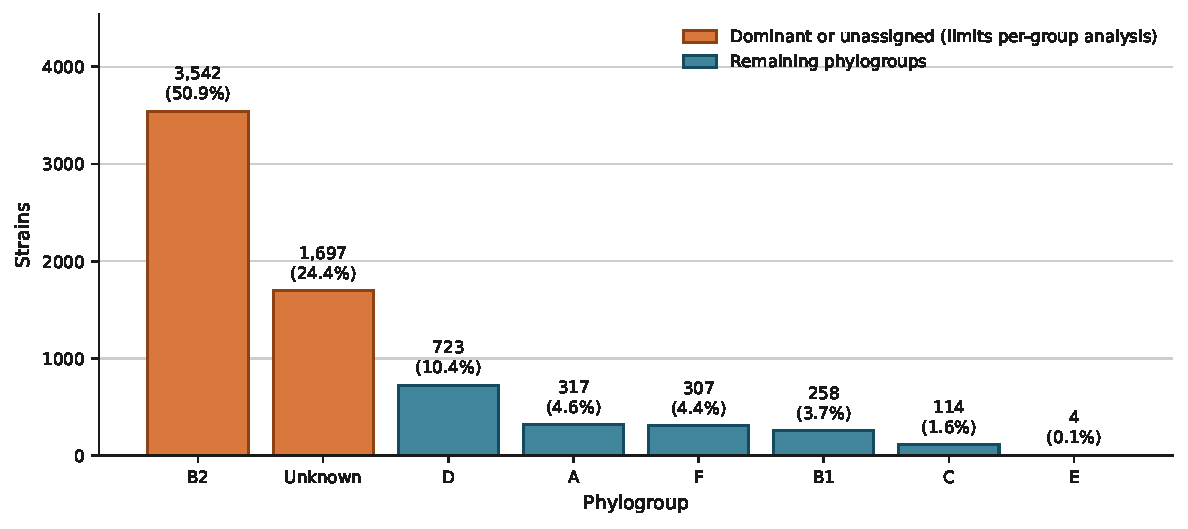
\includegraphics[width=0.94\textwidth]{fig_population_structure.pdf}
\caption{Phylogroup composition of the 6{,}962 strains.}
\label{fig:phylogroup_composition}
\fignote{The values of Table~\ref{tab:phylogroups} drawn to scale: a split by
phylogroup is largely a split of B2 against everything else.}
\end{figure}

\FloatBarrier
\subsection{Data Integration}

We had two checks before training. The three feature matrices were of different files. They
were also produced in various stages. We therefore made sure that they had the same strains in
the same order. We also verified that they were using the same names of genes. The first confirmed that the ordering of all 6,962 strain identifiers is
identical in all views; otherwise, one genome's SNPs would be paired with another genome's
genes.

\vspace{1em}

The latter one discovered a real challenge. None of the genes were found in common when the
gene identifiers in the SNP views were compared to the presence and absence view, because the
PLINK reader had created its own placeholder names for the genes and not read the actual gene
identifiers from the annotation file. Once the reader was corrected, all 5,000 genes chosen for
the SNP views were found in the 32,441-gene catalogue, a 100 per cent overlap. Nothing would have
failed visibly had this check not been run. The model would have received views labelled with the
wrong gene names, and the gene-level reading from Section~\ref{subsec:attnfix} would have been
comparing labels with no meaning against one another. Both the checks are now programmed as a
fixed step prior to any training run.

\FloatBarrier
\subsection{Data Reduction}

There are 535,439 features for 6,962 strains (some 77 candidate features for each sample). So,
it was not an optimisation to reduce the feature space. It was necessary for modelling, for the
reason explained in Section~\ref{subsec:hybrid}. The features were reduced at the gene level
rather than at the individual-variant level as the model operates at the gene level. Lastly,
only the genes that survived the two filters were retained. If a gene has fewer variable
positions, we cannot support a within-gene pattern, which is what our first view is designed to
find; thus the variability filter retains a gene if it has five or more SNPs across the
collection. After this step, 13,799 of the 18,975 genes in the matrix remain. These genes are
then sorted by importance in the gradient boosting model~\cite{chen2016xgboost} using the
importance filter. That model is trained separately for each of the seven antibiotics.
First, we filtered each set of SNPs with a chi-squared pre-filter and kept the top 50,000 per
drug, and trained a single XGBoost model for each antibiotic on its respective chi-squared
filtered subset, calculating each gene's cumulative gain for each model. The final importance
score for each gene is the sum of the per-antibiotic importance over all seven models, and the
5,000 most important (highest summed) genes are retained.

\vspace{1em}

The two filters were fitted solely based on the training partition. This is quite easy to
forget, and quite hard to do well: had the test labels been visible during ranking, they would
have changed what features exist in the first place, and each score in
Chapter~\ref{ch:results} would then have been overoptimistic by an unknown amount. Figure~\ref{fig:gene_feature_space} shows how
much the gene feature space is reduced by the two filters used above.

\begin{figure}[htb]
\centering
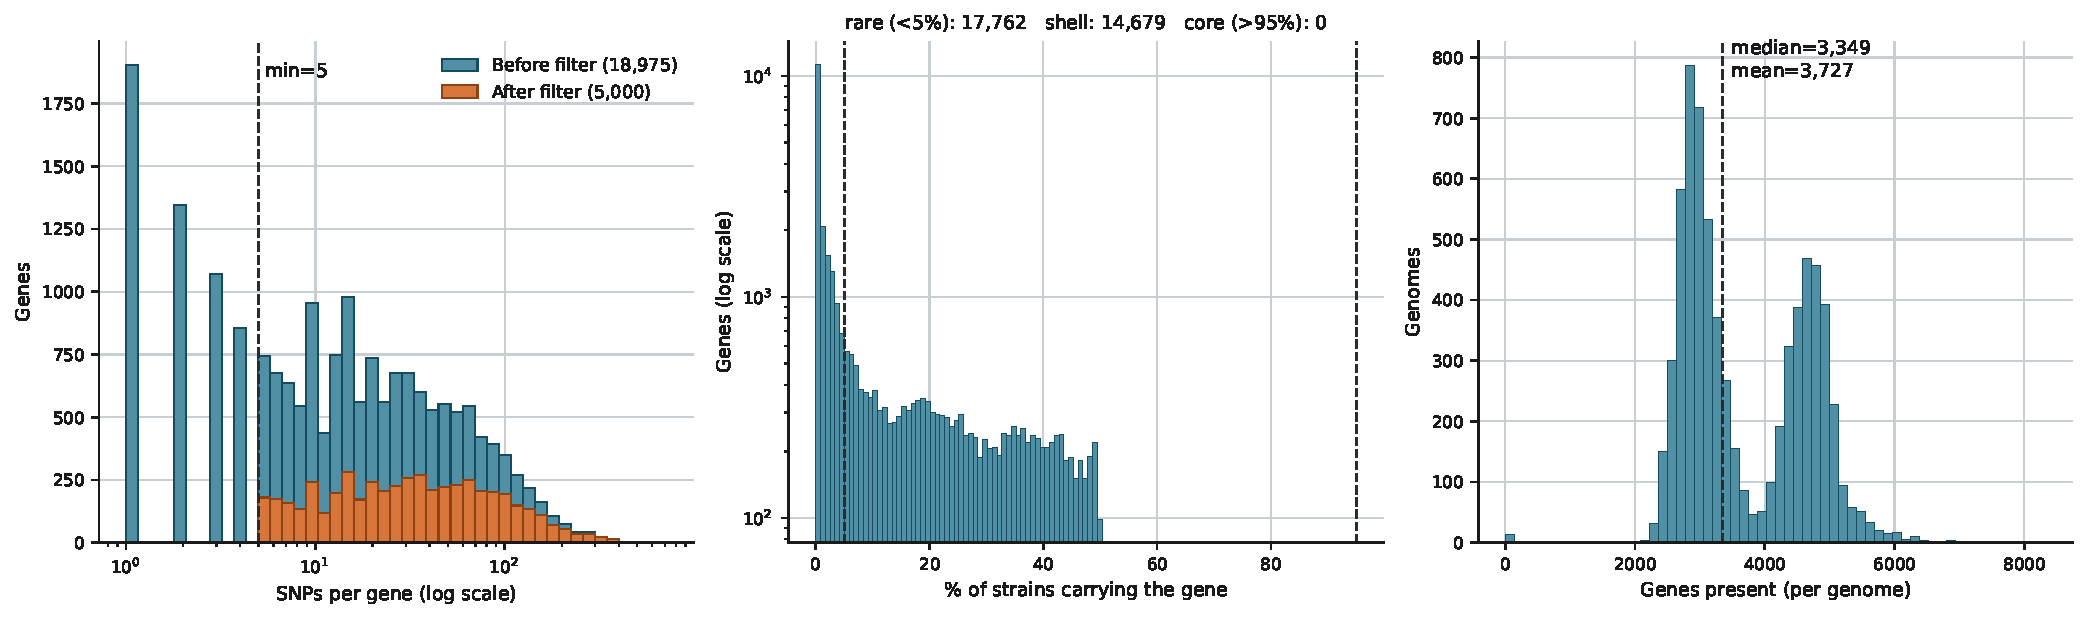
\includegraphics[width=\textwidth]{fig_gene_feature_space.pdf}
\caption{The gene feature space before and after filtering.}
\label{fig:gene_feature_space}
\fignote{\textbf{Left:} SNPs per gene across the 18{,}975 genes of the SNP view,
before and after the variability and importance filters cut them to 5{,}000.
\textbf{Centre and right:} the separate 32{,}441-gene presence and absence
catalogue, which is mostly rare genes: 17{,}762 are carried by under 5\% of strains
and none by more than 95\%, and a typical genome holds a median of 3{,}349 of them
against a mean of 3{,}727.}
\end{figure}

After filtering, 5,000 genes remain. These genes contain 262,225 SNPs. This corresponds to
approximately 49.0\% of the original variants. These genes differ widely in size: the smallest carries 5 SNPs, the median
32, the mean 52, and the largest 717. That distribution fed one last decision. Our first view
reads each gene as a fixed length block, which we set to 64 positions. Approximately 28\% of
the selected genes are longer than 64 SNPs and are truncated, the remaining genes are padded
with zeros and masked with zeros, so the padding does not contribute. A gene block has an
average of 35 positions out of 64 that are occupied by real positions. Most genes would waste
memory if the block were too long, while a shorter block would cause the median gene to be
cut.

\FloatBarrier
\subsection{Preprocessed Data and the Three Evaluation Splits}
\label{subsec:splits}

The splits determine what a score measures, because of which we give a detailed account of
how we split the data. Approximately 15 percent of each split is for testing, another 15
percent of each split is for validation, and approximately 70 percent is for training. The
test set is never used in the model selection or tuning; it is not touched until the final
evaluation, and every split has been performed with the same fixed random seed (42), which
means that any number reported in this research can be exactly re-generated by running the same
code. We constructed three splits and they address three questions.
Table~\ref{tab:splits} gives their sizes and
Figure~\ref{fig:split_composition} draws the same three partitions as bars, so
that the one split whose training and validation sizes are not round can be seen at
a glance.

\vspace{1em}

The random split assigns strains via shuffling, stratified on the ampicillin label to achieve
class balance across the three sets. This results in a training set of 4,872 strains, a
validation set of 1,045 and a test set of 1,045. It is the normal setting, and the one that is
used in the majority of published work; the related strains can fall on both sides, and do.
The partition sizes remain the same but the partition balancing takes into account the
eight-way phylogroup assignment, each lineage group being represented in each of the three
sets in the same proportion as it would be in the collection as a whole. This does not control
class balance.

We just want to clarify what this second split is, as it can be very easily inflated. It is a
stratified split, as opposed to a holdout. By design, every phylogroup appears on both sides so
it is not testing how the model performs on a lineage it has never seen before. What it tests
is the extent to which the result is influenced by the choice of stratification variable. This
is a weaker question than the one we wished to answer, and Section~\ref{sec:discussion} tells
what happened when we first treated it as one that answered the stronger question.

The train/test split answering that more stringent question is the sequence-type lineage
holdout, and is the one upon which the central result of this research is built, so we will
describe its construction in full. Strains each have a multi-locus sequence type, a generic
label in bacterial genomics that clusters strains based on shared descent in the recent past
and is much more specific than phylogroup. We extracted it from the metadata provided on
strains, and rather than assigning sequence type by the position or row in the genome table, we
mapped the metadata identifying number to recover a sequence type for the large majority of the
collection.

Two rules were set prior to examining any result. In the absence of a sequence type, any
strain was assigned to training as an unlabelled group cannot be held out safely. If the
number of sequences in a collection type was more than five percent, then it was also put in
training. The other rule is equally important. Type 73 represents approximately an eighth of the entire
dataset. If that clone has a relatively large number of different strains found in the test
set, the test will mostly be measuring this particular clone. This does not measure how well
the model will work on novel lineages. The rest of the sequence types were then allocated
whole to training, validation or test by a seeded permutation walk which successively adds
groups until the desired proportion of genomes in each partition is reached.
Figure~\ref{fig:st_distribution} shows the size distribution these rules had to work around.

\begin{figure}[htb]
\centering
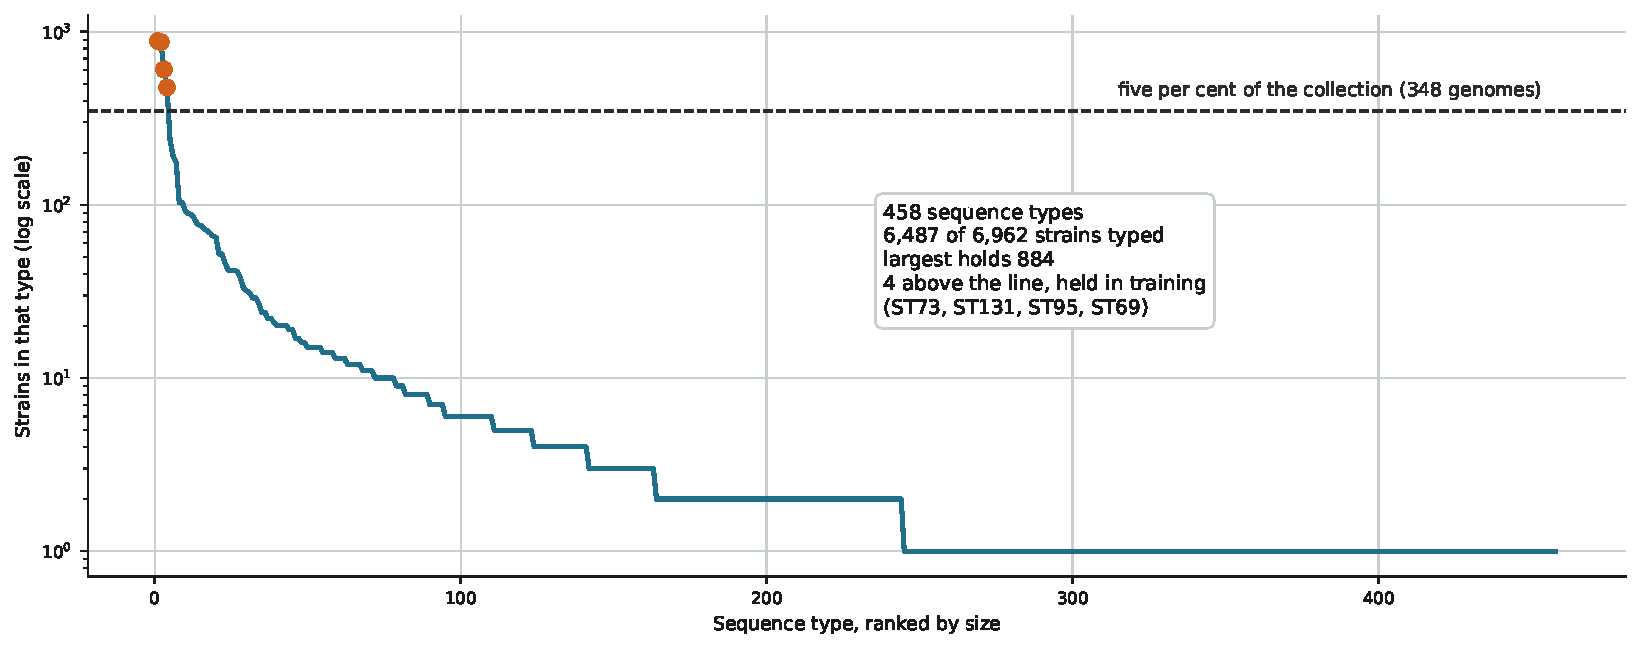
\includegraphics[width=\textwidth]{fig_st_distribution.pdf}
\caption{The 458 sequence types, ranked by size.}
\label{fig:st_distribution}
\fignote{A few types are very large and most are very small. The largest holds 884
strains, nearly one genome in eight, and four types sit above five per cent of the
collection. Those four, ST73, ST131, ST95 and ST69, are placed in training, so that
no test set can be dominated by a single clone.}
\end{figure}

We kept whole groups in the same partition. Owing to this, there are no ideal percentages of
the split. A chance division would appear less lopsided. This effect is reflected in our data
split as well. The holdout uses a training set of 4,836 strains, a
validation set of 1,081 and a test set of 1,045. No sequence type was observed to be present in
more than one partition (as opposed to assuming this), and Section~\ref{subsec:prevmatch}
describes an almost identical scan of the resulting test set, with no duplicate sequence types
found. The same point of method is used for all 3 splits. This 5,000 gene selection mentioned
earlier in this section under Data Reduction is re-fitted on each split's training partition
instead of being computed only once and used for each split. The definition of the pipeline
used an earlier version that leaked information between splits, which was fixed prior to any
results in this research. Refitting per split indicates that each split generates its ranking of
informative genes. It comes as a surprise to note that the holdout's gene set overlaps the
random split's by less than half, indicating that the resistance signal is not located in a
few genes but in many genes that are partly interchangeable.

\begin{table}[htb]
\centering
\caption{The three evaluation splits and the partition sizes they produce. Only the
third assigns whole groups, which is why its training and validation sizes are not
round.}
\label{tab:splits}
\small
\begin{tabular}{|l|l|r|r|r|}
\hline
\textbf{Split} & \textbf{Balanced on} & \textbf{Train} & \textbf{Val} & \textbf{Test} \\
\hline
Random & Ampicillin label & 4{,}872 & 1{,}045 & 1{,}045 \\ \hline
Phylogroup-stratified & Eight-way phylogroup & 4{,}872 & 1{,}045 & 1{,}045 \\ \hline
Sequence-type holdout & Whole sequence types, none shared & 4{,}836 & 1{,}081 & 1{,}045 \\ \hline
\end{tabular}
\vspace{0.4em}

\noindent\footnotesize\textit{Note:} Every row sums to 6{,}962. Only the sequence-type holdout
assigns whole groups at a time, which is why its training and validation partitions are not
round numbers; its test partition happens to land on the same 1{,}045 as the other two.
\end{table}

\begin{figure}[htb]
\centering
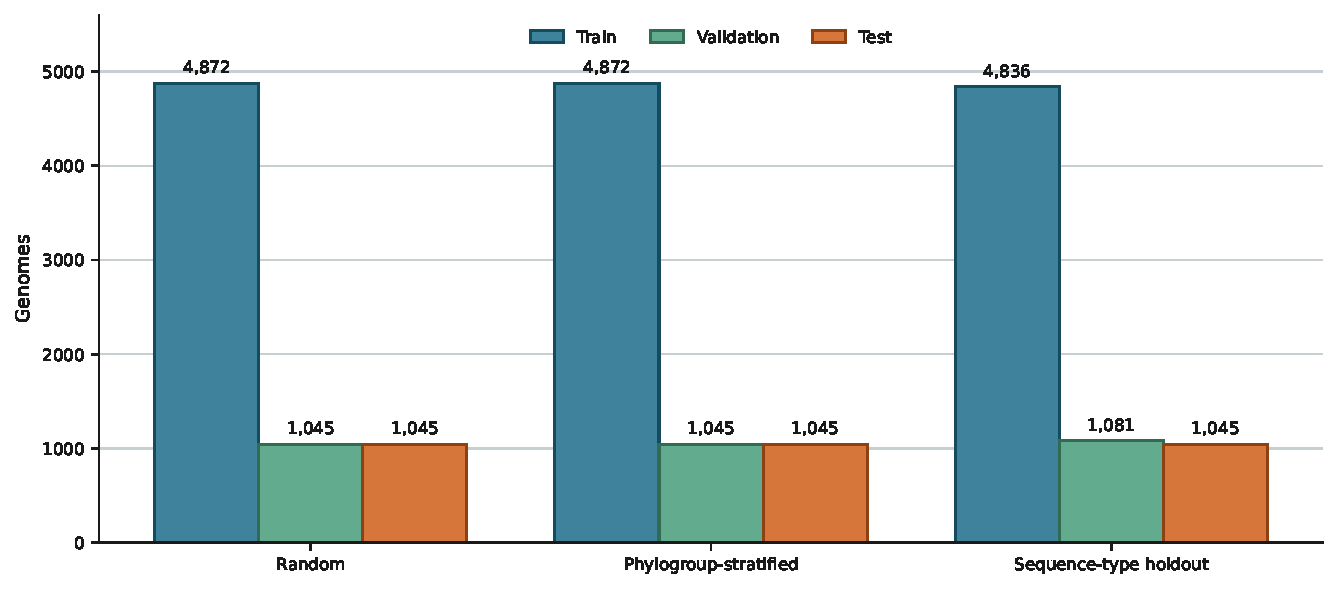
\includegraphics[width=\textwidth]{fig_split_composition.pdf}
\caption{Train, validation and test sizes for the three splits of
Table~\ref{tab:splits}.}
\label{fig:split_composition}
\fignote{The same 6{,}962 genomes are partitioned three different ways. Only the
sequence-type holdout keeps whole groups together, which is why its training and
validation partitions are not round.}
\end{figure}

For each split we also record the number of labelled strains and the resistance prevalence in
each partition, per antibiotic. The lower bound of precision recall AUC will be determined by
prevalence, meaning that a lower prevalence will result in a lower score even if the model is
equally good. The effects are greatest for the holdout, as forcing the largest clones into
training causes a shift in prevalence downwards for all of the antibiotics. Reporting the
prevalence with the score enables a reader to distinguish a drop because of a tougher test set
from a drop because of a lower floor. Figure~\ref{fig:split_prevalence_shift} shows how
large that shift is for each split.

\begin{figure}[htb]
\centering
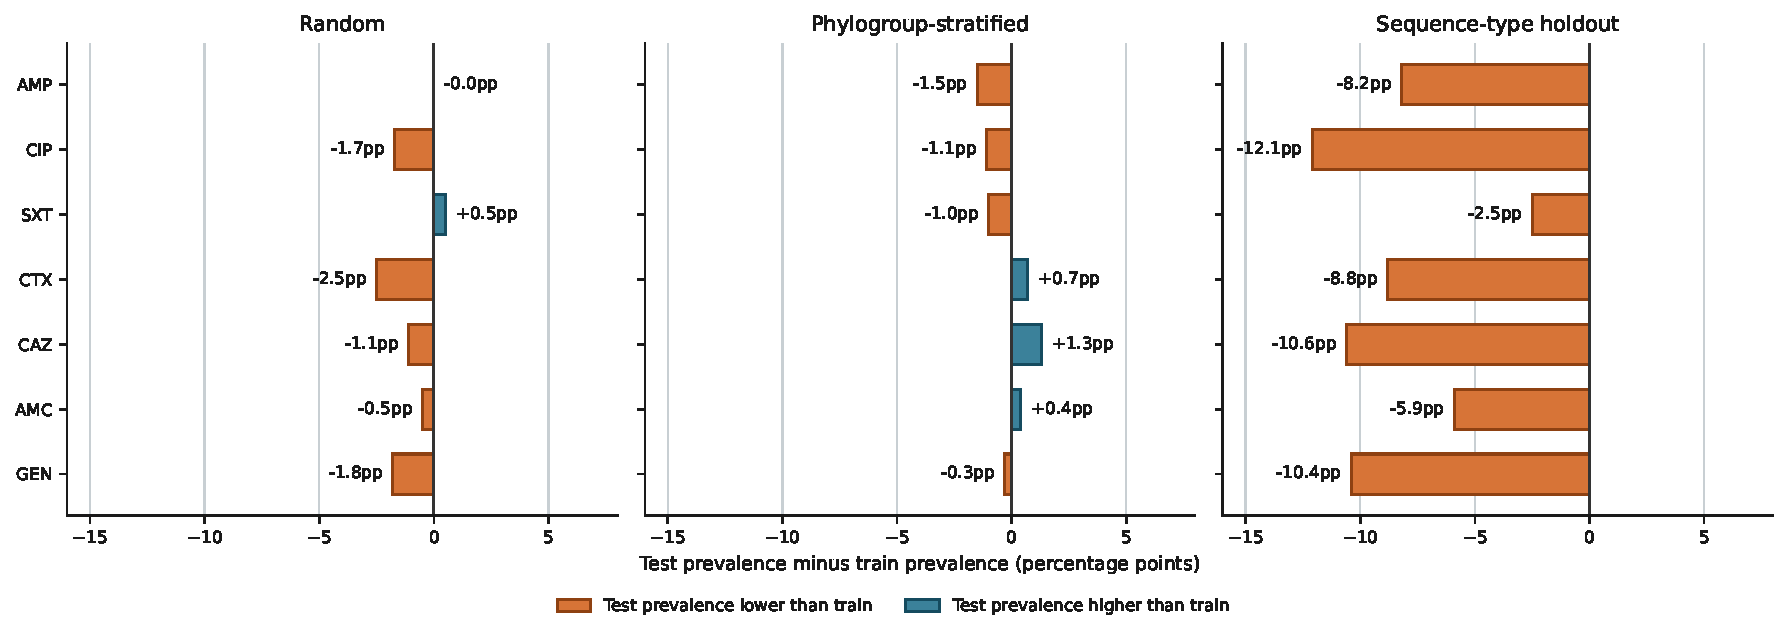
\includegraphics[width=\textwidth]{fig_split_prevalence_shift.pdf}
\caption{Test-minus-train resistance prevalence, in percentage points, per
antibiotic and per split.}
\label{fig:split_prevalence_shift}
\fignote{The random and phylogroup-stratified splits stay within 2.5 points and move
in both directions. The sequence-type holdout moves downwards for every antibiotic,
by 2.5 to 12.1 points, and since the no-skill floor of precision recall AUC is the
prevalence itself, part of the drop reported in Chapter~\ref{ch:results} follows from
this shift rather than from the model.}
\end{figure}

Now combining the three genomic views with the encoding of the phylogroup, the labels and
their mask provides the six arrays that are actually passed to the model, which are contained
in Table~\ref{tab:views}.

\begin{table}[htb]
\centering
\caption{Arrays produced by the preprocessing pipeline: four feature
representations, followed by the label matrix and its mask.}
\label{tab:views}
\small
\begin{tabular}{|l|l|l|l|}
\hline
\textbf{Representation} & \textbf{Shape} & \textbf{Type} & \textbf{What it captures} \\
\hline
SNP blocks by gene    & $6{,}962 \times 5{,}000 \times 64$ & int8    & mutation patterns inside genes \\ \hline
Gene presence/absence & $6{,}962 \times 32{,}441$          & uint8   & genes acquired from elsewhere \\ \hline
Per-gene statistics   & $6{,}962 \times 5{,}000 \times 4$  & float32 & coarse gene-level variation \\ \hline
Phylogroup one-hot    & $6{,}962 \times 8$                 & float32 & broad lineage \\ \hline
Labels                & $6{,}962 \times 7$                 & bool    & resistant or susceptible \\ \hline
Label mask            & $6{,}962 \times 7$                 & bool    & which labels were measured \\ \hline
\end{tabular}
\vspace{0.4em}

\noindent\footnotesize\textit{Note:} These six arrays are everything the model receives. The
mask is what allows an untested strain and drug combination to be skipped rather than imputed.
\end{table}

Two characteristics of this data set set the stage for everything that follows. It is broad
and short: there are still far more features than strains even after dimensionality reduction,
so the design favors gradient boosting over a large network. And it is patchy: antibiotic
coverage ranges from 49 to 87 per cent according to drug while prevalence ranges from 12 to 50
per cent, meaning no averaged score across the seven antibiotics serves it well; hence each
result in Chapter~\ref{ch:results} is reported per drug, as well as on average.

\vspace{1em}

A single collection does not provide an answer to the question of whether or not an approach
travels. We use a second, independent set of \textit{E. coli} genomes that were collected at
the University of Giessen and published by Ren et al.~\cite{Ren2022}. Isolates were from human
and animal clinical specimens and susceptibility was done by automated testing and interpreted
according to EUCAST breakpoints. Ren et al.\ report 987 Giessen isolates in total
(Table~\ref{tab:summary}); the subset we use is the 809 that carry a complete
result for all four of the antibiotics shared with our panel, which is the same
809 used by Siddiqui and Tarannum~\cite{siddiqui2025amrensemble}. Those 809
strains are described by 60,936 SNP positions each. Its composition is shown in
Table~\ref{tab:giessen}.

\begin{table}[htb]
\centering
\caption{Composition of the external Giessen dataset.}
\label{tab:giessen}
\small
\begin{tabular}{|l|r|r|r|}
\hline
\textbf{Antibiotic} & \textbf{Resistant} & \textbf{Susceptible} & \textbf{Prevalence} \\
\hline
CIP & 366 & 443 & 0.452 \\ \hline
CTX & 358 & 451 & 0.443 \\ \hline
CAZ & 276 & 533 & 0.341 \\ \hline
GEN & 188 & 621 & 0.232 \\ \hline
\end{tabular}
\vspace{0.4em}

\noindent\footnotesize\textit{Note:} Every isolate carries a result for all four drugs, so no
mask is needed here. Prevalence is roughly two to three times the Arcadia value for the same
drug, which is why the retention figures in Chapter~\ref{ch:results} cannot be read as
like-for-like.
\end{table}

There are two disparities with the Arcadia data that influence its use. The first one is the
reference. In Giessen variants are listed in order of a single reference genome (columns are
ordered along the chromosome) while Arcadia uses a pan-genome (the ordering of the columns has
no meaning). This difference is not an inconvenience: it makes the locality test in
Section~\ref{subsec:cnnfail} possible because we have one set of data for which locality
should matter, and one set for which it should not. The second is the two feature spaces have
no overlap. The model trained on Arcadia cannot be used at Giessen, since there is no shared
feature vector, so anything we do across the two collections must be a comparison of methods,
as Section~\ref{sec:comparisons} states.

\vspace{1em}

Also, there is a difference in the label names. The Giessen phenotypes are interpreted against
the EUCAST breakpoints, and the Arcadia phenotypes are interpreted according to a different
standard. Breakpoint differences between the two also exist for the same drug, and this could
contribute to performance differences between collections, and not only to the model. We are
unable to separate the two effects with the data available and designate it as a limitation
for any cross-collection comparison. This dataset consists of 809 strains with results for all
four types of drugs, unlike Arcadia where some of the labels are missing, so masking is not
necessary. The numbers were randomly split by ciprofloxacin into 647 for training, 81 for
validation and 81 for testing. The test partition is small and that is why the Giessen
confidence intervals in Chapter~\ref{ch:results} are wider than those for Arcadia.

\FloatBarrier
\section{Implementation of Selected Design}
\label{subsec:common_framework}

All of the settings below are global across the model. Most follow traditional practice and
are therefore included for completeness; a few are less obvious and are explained, where
necessary.

\subsection{Binary Classification Setup}

In the case of each antibiotic, the model aims to predict either resistance (labelled 1) or
susceptibility (labelled 0). The inputs are the three genomic views discussed in the top-level
overview and each raw score is transformed into a probability using the logistic sigmoid from
Equation~\eqref{eq:sigmoid}. All seven antibiotics are predicted in the same forward pass,
making it a multi-label problem instead of a multi-class problem: a strain may be resistant to
multiple drugs simultaneously and the predictions do not have to compete with each other.

\subsection{Handling Class Imbalance}

Susceptible strains by far outnumber resistant ones for various drugs, which poses a very real
trap: a model predicting susceptible in all cases scores highly on accuracy and is useless,
but which is approximated well by a model that predicts the majority class as the easiest way
to minimize the loss.

To avoid this, the resistant and susceptible samples are reweighted in inverse proportion to
their frequency of occurrence, such that a mistake in getting a rare resistant strain is much
costlier. In the classical tree-based learners it can be accomplished by the
\texttt{scale\_pos\_weight} parameter,
\begin{equation}
\text{\texttt{scale\_pos\_weight}} = \frac{N_{\text{neg}}}{N_{\text{pos}}},
\label{eq:scale_pos_weight}
\end{equation}
where $N_{\text{neg}}$ and $N_{\text{pos}}$ are the numbers of susceptible and resistant
samples. In Logistic Regression and Random Forest, this is accomplished by using balanced
class weights, and in the neural lenses, by using positive class weighting in the loss. For
this reason, we use precision-recall AUC and not accuracy during the evaluation as accuracy
would conceal precisely the failure we want to avoid.

\subsection{Data Splitting Strategy}

The model is trained and tested in three settings which are generated in
Section~\ref{subsec:splits}: random split, phylogroup-stratified split, and sequence-type
lineage holdout. The reporting of all three, and the space between them, is part of the
evaluation design. A validation set is employed for tuning; a final test set is only employed
for the final evaluation and a fixed random seed of 42 is used throughout.

\subsection{Threshold Selection}
\label{subsec:threshold_selection}

To arrive at the final decision, we use a constant probability threshold of 0.5 for each of the
antibiotics, as in Equation~\eqref{eq:decision}. This is the indifferent option. It places the same emphasis on the two kinds of errors. But in
clinical practice this is not the case. The issue of predicting a resistant strain as being
susceptible can result in administering a drug that is not effective. The reverse error is
only going to result in picking another drug.
A recall-oriented adjustment was made according to the $F_{\beta}$ score,
\begin{equation}
F_{\beta} = \frac{(1 + \beta^2)\cdot\text{Precision}\times\text{Recall}}{\beta^2\cdot\text{Precision} + \text{Recall}},
\label{eq:fbeta}
\end{equation}
with $\beta = 2$ to give four times as much weight to recall as to precision, would lower the
threshold and capture more resistant strains while increasing the number of false alarms. To
avoid tuning the numbers in our favour, all headline results in this research have been reported
at the neutral threshold of 0.5 and then per-antibiotic threshold tuning has been directly
tested in Section~\ref{sec:perfeval}, fitting the threshold on validation and applying it to
test.

\FloatBarrier
\subsection{Optimization and Training Schedule}

The training of the neural lenses, the gate and the fusion step is done in a simultaneous way,
so that each lens learns to be useful in conjunction with the others and not optimised alone.
The objective consists of three terms: a binary cross-entropy loss over the fused scores, the
entropy regulariser in Equation~\eqref{eq:entropy_reg}, and an auxiliary loss on each lens. This extra loss term is important. In its absence, a lens which is momentarily disregarded by
the gate achieves extremely limited gradient. This leads to its cessation of improvement. This
problem is avoided by the auxiliary loss. It aids all lenses in continuing to learn, even when
they are not being selected by the gate. Optimization
employs the AdamW optimiser that keeps the weight decay and gradient update decoupled, and the
learning rate of $10^{-3}$, annealed on a cosine schedule over the epoch budget, weight decay
of $10^{-4}$, batch size of 16, gradient clipping of norm 1.0, and mixed-precision training,
with up to 50 epochs and early stopping after 8 consecutive no-improvement epochs of
validation mean precision-recall AUC. The inclusion of gradient clipping is because, when
attention is placed over 32{,}441 genes, the gradients can sometimes be quite large, causing
the training to become unstable. The five classical base learners are trained individually via
5-fold cross validation, with out-of-fold predictions, which are then used to fit the
logistic-regression meta-learner, along with the neural probabilities. The most important
hyperparameters are summarised in Table~\ref{tab:hyperparameters}.

{\small\setlength{\tabcolsep}{5pt}
\begin{longtable}{|>{\raggedright\arraybackslash}p{2.9cm}|>{\raggedright\arraybackslash}p{10.7cm}|}
\caption{Hyperparameter configuration for the classical base learners and the neural model.}
\label{tab:hyperparameters}\\
\hline
\textbf{Component} & \textbf{Key Hyperparameters} \\
\hline
\endfirsthead
\hline
\textbf{Component} & \textbf{Key Hyperparameters} \\
\hline
\endhead
\hline
\multicolumn{2}{r}{\footnotesize\textit{Continued on the next page}}\\
\endfoot
\hline
\endlastfoot
XGBoost (gene) &
n\_estimators=1500; max\_depth=5; min\_child\_weight=5; learning\_rate=0.05;
subsample=0.8; colsample\_bytree=0.7; reg\_alpha=0.1; reg\_lambda=1.0; gamma=0.1;
tree\_method='hist'; scale\_pos\_weight=$N_-/N_+$ per drug; early\_stopping\_rounds=150 \\ \hline
XGBoost (raw) &
chi\textsuperscript{2}-prefilter (top 50{,}000 SNPs); n\_estimators=1500; max\_depth=5;
learning\_rate=0.05; subsample=0.8; colsample\_bytree=1.0; colsample\_bynode=0.5;
reg\_alpha=0.1; reg\_lambda=1.0; tree\_method='hist'; scale\_pos\_weight=$N_-/N_+$ per drug;
early\_stopping\_rounds=150 \\ \hline
LightGBM &
n\_estimators=1500; num\_leaves=63; max\_depth=6; min\_child\_samples=20; learning\_rate=0.05;
subsample=0.8; subsample\_freq=1; colsample\_bytree=0.7; reg\_alpha=0.1;
reg\_lambda=1.0; scale\_pos\_weight=$N_-/N_+$ per drug; early\_stopping\_rounds=150 \\ \hline
Random Forest &
n\_estimators=200; max\_depth=12; min\_samples\_leaf=10 \\ \hline
Logistic Regression (base) &
scikit-learn defaults (L2 penalty) \\ \hline
Neural lenses + MoE gate &
optimizer=AdamW; learning\_rate=$10^{-3}$ with cosine annealing;
weight\_decay=$10^{-4}$; batch\_size=16;
epochs=50; patience=8; grad\_clip=1.0; mixed precision; entropy weight=0.01; seed=42 \\ \hline
Stacking meta-learner &
Logistic Regression (L2, $C=1.0$), per antibiotic; 5-fold out-of-fold inputs \\ \hline
\end{longtable}}